
\section{Diseño}

En esta sección se muestra el diseño del sistema que será implementado, los diagramas de los procesos que se llevarán a cabo, los diagrmas de actividades y UML,esta sección se divide en dos secciones, el diseño del reconocimiento de voz y el diseño de la aplicación.

\subsection{Diseño del reconocimiento de voz}

De acuerdo a lo visto en la sección de análisis en la Figura \ref{fig:SRgeneral} se muestra el diagrama general del reconocimiento de voz que será implementado para llevar a cabo el reconocimiento de las palabras a ser traducidas al lenguaje de señas.

		\begin{figure}[H]
			\centering
			
\includegraphics[width=1\linewidth]{figures/srGeneral}
			\caption{Diagrama general del reconocimiento de voz.}
			\label{fig:SRgeneral}
		\end{figure}
		
\subsubsection*{Pre-procesamiento}		

El pre-procesamiento de la señal de voz se llevará a cabo de acuerdo al diagrama de la  Figura \ref{fig:preprocesamientoDes}, esta étapa consta de cuatro bloques que se explican a continucación.

		\begin{figure}[H]
			\centering
			
\includegraphics[width=1\linewidth]{figures/preprocesamientoDes}
			\caption{Diagrama de la etapa de pre-procesamiento.}
			\label{fig:preprocesamientoDes}
		\end{figure}
		
	\begin{itemize}
		\item	\textbf{Detección de bordes y separación de palabras:} esta etapa llevará a cabo la detección de bordes de las palabras invlucradas en la oración (señal de voz a reconocer) ya que se tratarán con frases y el número de palabras puede variar. De acuerdo a la sección del análisis, se hará uso del algoritmo que aprovecha las características de energía de señal y tasa de cruces por cero del dominio del tiempo y el centroide y flujo espectral del dominio frecuencial propuesto en \cite{A31}, una vez segmentada la frase en palabras, cada señal de voz correspondiente a una palabra será procesada de forma individual.
		\item	\textbf{Filtro preénfasis:} el filtro aplicado será un filtro digital de primer orden y de acuerdo al análisis el coeficiente $a$ de la ecuación $\hat{s}(n)=s(n)-a\cdot s(n-1)$ será igual a $0.95$.
		\item	\textbf{Segmentación:} la segmentación de la señal de voz se realizará con una duración de 40 ms del segmento y un traslape de 20 ms.
		\item	\textbf{Aplicación de ventana:} finalmente se aplicará la ventana de Hamming de acuerdo al análisis hecho en la sección anterior.
	\end{itemize}
	
	\subsubsection*{Extracción de características}
	
	La señal resultante del pre-procesamiento sirve de entrada al bloque de extracción de características, para la extracción de características se ha decidido realizar por medio de los MFCC que se realiza de acuerdo a la Figura \ref{fig:extraccionMFCC}.
	
		\begin{figure}[H]
			\centering
			
\includegraphics[width=1\linewidth]{figures/extraccionMFCC}
			\caption{Cálculo de los coeficientes MFCC.}
			\label{fig:extraccionMFCC}
		\end{figure}

	\subsubsection*{Red neuronal}
		
	La red neuronal que se implementará para llevar a cabo el reconocimiento de patrones será una arquitectura \textit{feedforward Pattern Recognition} y será entrenada con el algoritmo de entrenamiento \textit{Scaled Conjugate Gradient backpropagation} y como función de activación para la capa oculta se usará \textit{sigmoid} y en la capa de salida \textit{softmax}. Los vectores de entrada a la red serán los vectores de coeficientes cepstrales cuantizados vectorialmente, de esta forma se asegura una longitud fija de los vectores.

\subsection{Diseño de la aplicación}

En esta sección se muestra el diseño de la aplicación móvil mediante diagramas y el boceto de ésta. Los diagramas que se presentan son de casos de uso, de actividades, diseño de la base de datos y finalmente las pantallas de la aplicación, de esta forma se tendrá un mayor entendimiento de la secuencia de la aplicación y su estructuración.

\subsubsection{Diagrama de casos de uso}

Los siguientes diagramas junto con sus tablas muestran los casos de uso de la aplicación, así como los factores que intervienen.

En la Figura \ref{fig:casoUsoGen} se muestra un diagrama general de la aplicación mostrando el uso que puede hacer el usuario de la aplicación, en este caso son tres actividades principales: 

\begin{itemize}
\item	Traductor de voz a LSM.
\item	Síntesis de voz desde el teclado.
\item	Consulta de diccionario.
\end{itemize}

		\begin{figure}[H]
			\centering
			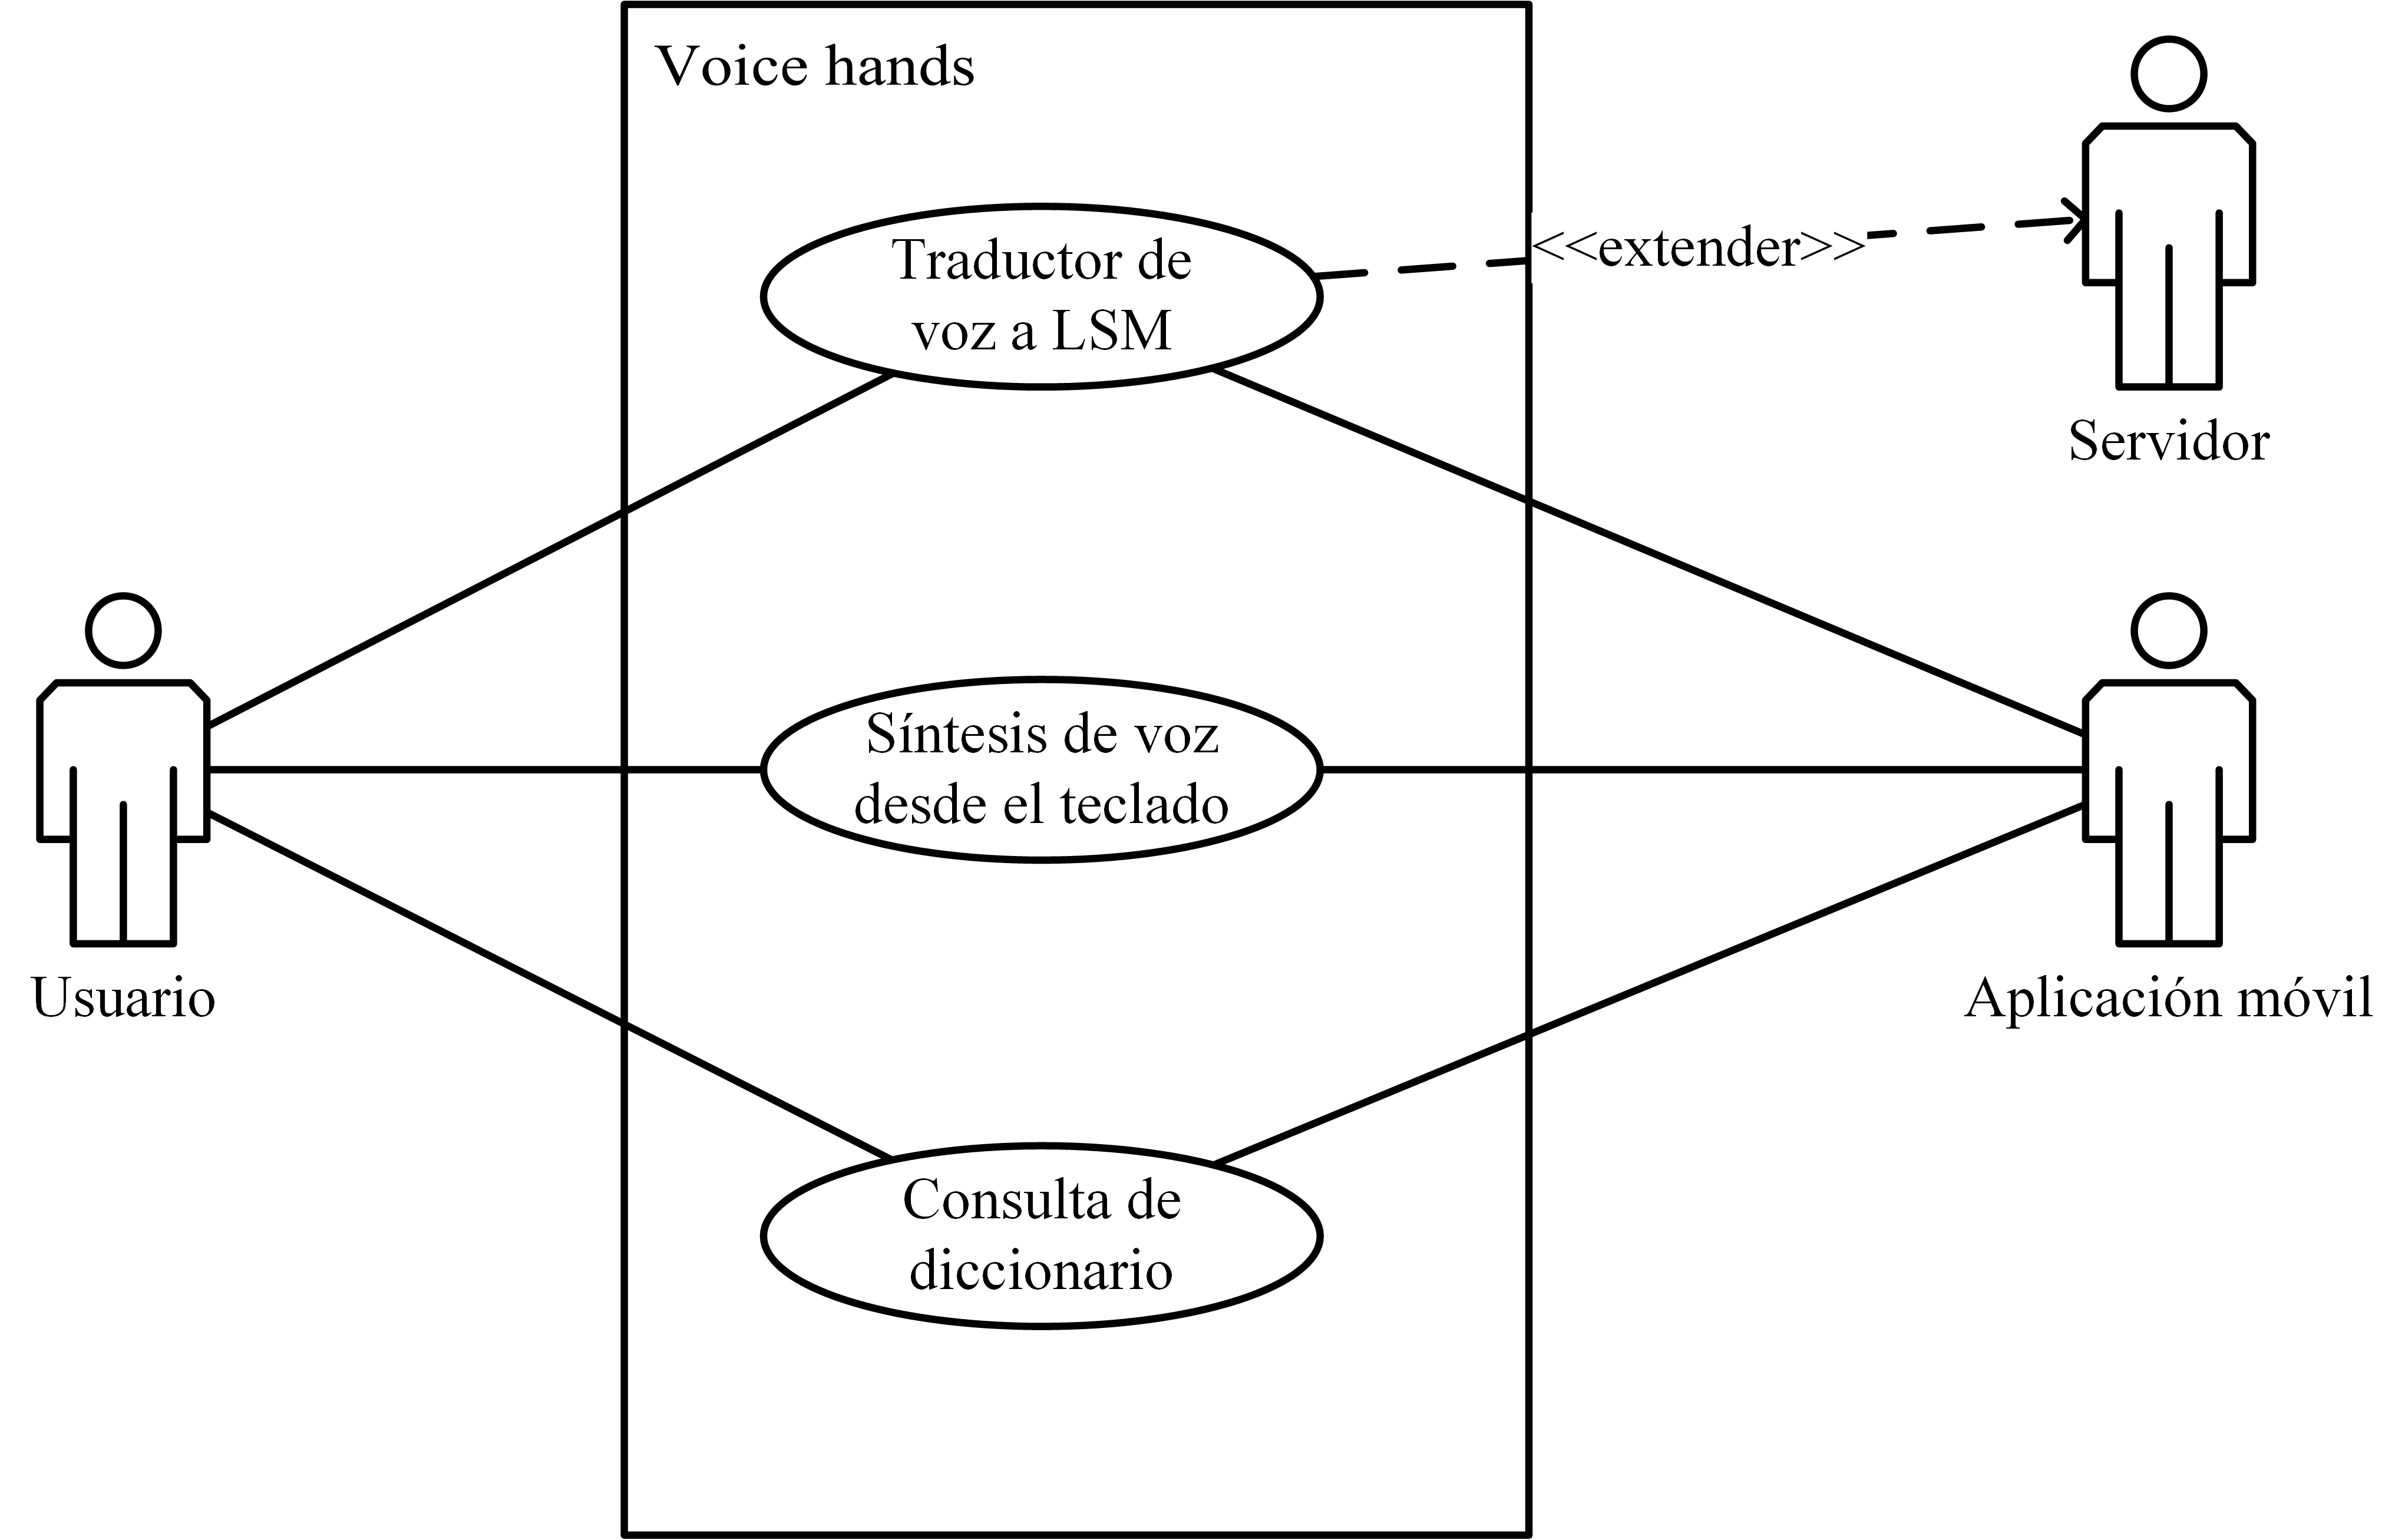
\includegraphics[width=0.8\linewidth]{figures/casoUsoGeneral}
			\caption{Caso de uso general}
			\label{fig:casoUsoGen}
		\end{figure}	
		
Como observamos, se cuenta con un tipo de usuario y del otro lado la opción del traductor hace uso del servidor para enviar y recibir información respecto a la frase grabada.

\paragraph{Traductor de voz a LSM}\paragraph{}

En la Tabla \ref{tb:casoUsoVoz} se muestra la especificación de la Figura \ref{fig:casoUsoVoz} correspondiente al caso de uso de traductor de voz a LSM, en este caso tenemos a un usuario que desea comunicarse con una persona que usa el LSM.		

\begin{table}[H]
\centering
\caption{Caso de uso \textit{``Traductor de voz''}}
\label{tb:casoUsoVoz}
\begin{tabular}{|l|l|}
\hline
\multicolumn{2}{|l|}{\cellcolor[HTML]{C0C0C0}Caso de uso: Traductor de voz a LSM}                                                                                                                                                                                                             \\ \hline
\multicolumn{2}{|l|}{Actor: Usuario, Aplicación móvil y Servidor}                                                                                                                                                                                                                             \\ \hline
\multicolumn{2}{|l|}{Descripción: Permite realizar la traducción del mensaje de voz grabado a LSM}                                                                                                                                                                                            \\ \hline
Curso normal                                                                                                                                            & Alternativas                                                                                                                        \\ \hline
\begin{tabular}[c]{@{}l@{}}1.	El usuario selecciona la función de \\ traductor\end{tabular}                                                             &                                                                                                                                     \\ \hline
\begin{tabular}[c]{@{}l@{}}2.	Deja presionado el botón de grabar \\ y se guarda el mensaje.\end{tabular}                                                &                                                                                                                                     \\ \hline
\begin{tabular}[c]{@{}l@{}}3.	Al terminar la grabación se envía al \\ servidor para su debido procesamiento.\end{tabular}                               & \begin{tabular}[c]{@{}l@{}}3.1.,Si no está disponible el servidor, se le \\ hará saber al usuario.\end{tabular}                     \\ \hline
\begin{tabular}[c]{@{}l@{}}4.	El servidor busca la palabra detectada \\ en la base de datos.\end{tabular}                                               & \begin{tabular}[c]{@{}l@{}}4.1.,Si no reconoce la palabra o no está en la \\ base de datos se le informará al usuario.\end{tabular} \\ \hline
\begin{tabular}[c]{@{}l@{}}5.	Se envía el resultado a la aplicación \\ móvil.\end{tabular}                                                              &                                                                                                                                     \\ \hline
\begin{tabular}[c]{@{}l@{}}6.	Se muestra en pantalla el resultado de \\ la traducción, así como también los \\ posibles mensajes de error.\end{tabular} &                                                                                                                                     \\ \hline
\end{tabular}
\end{table}

		\begin{figure}[H]
			\centering
			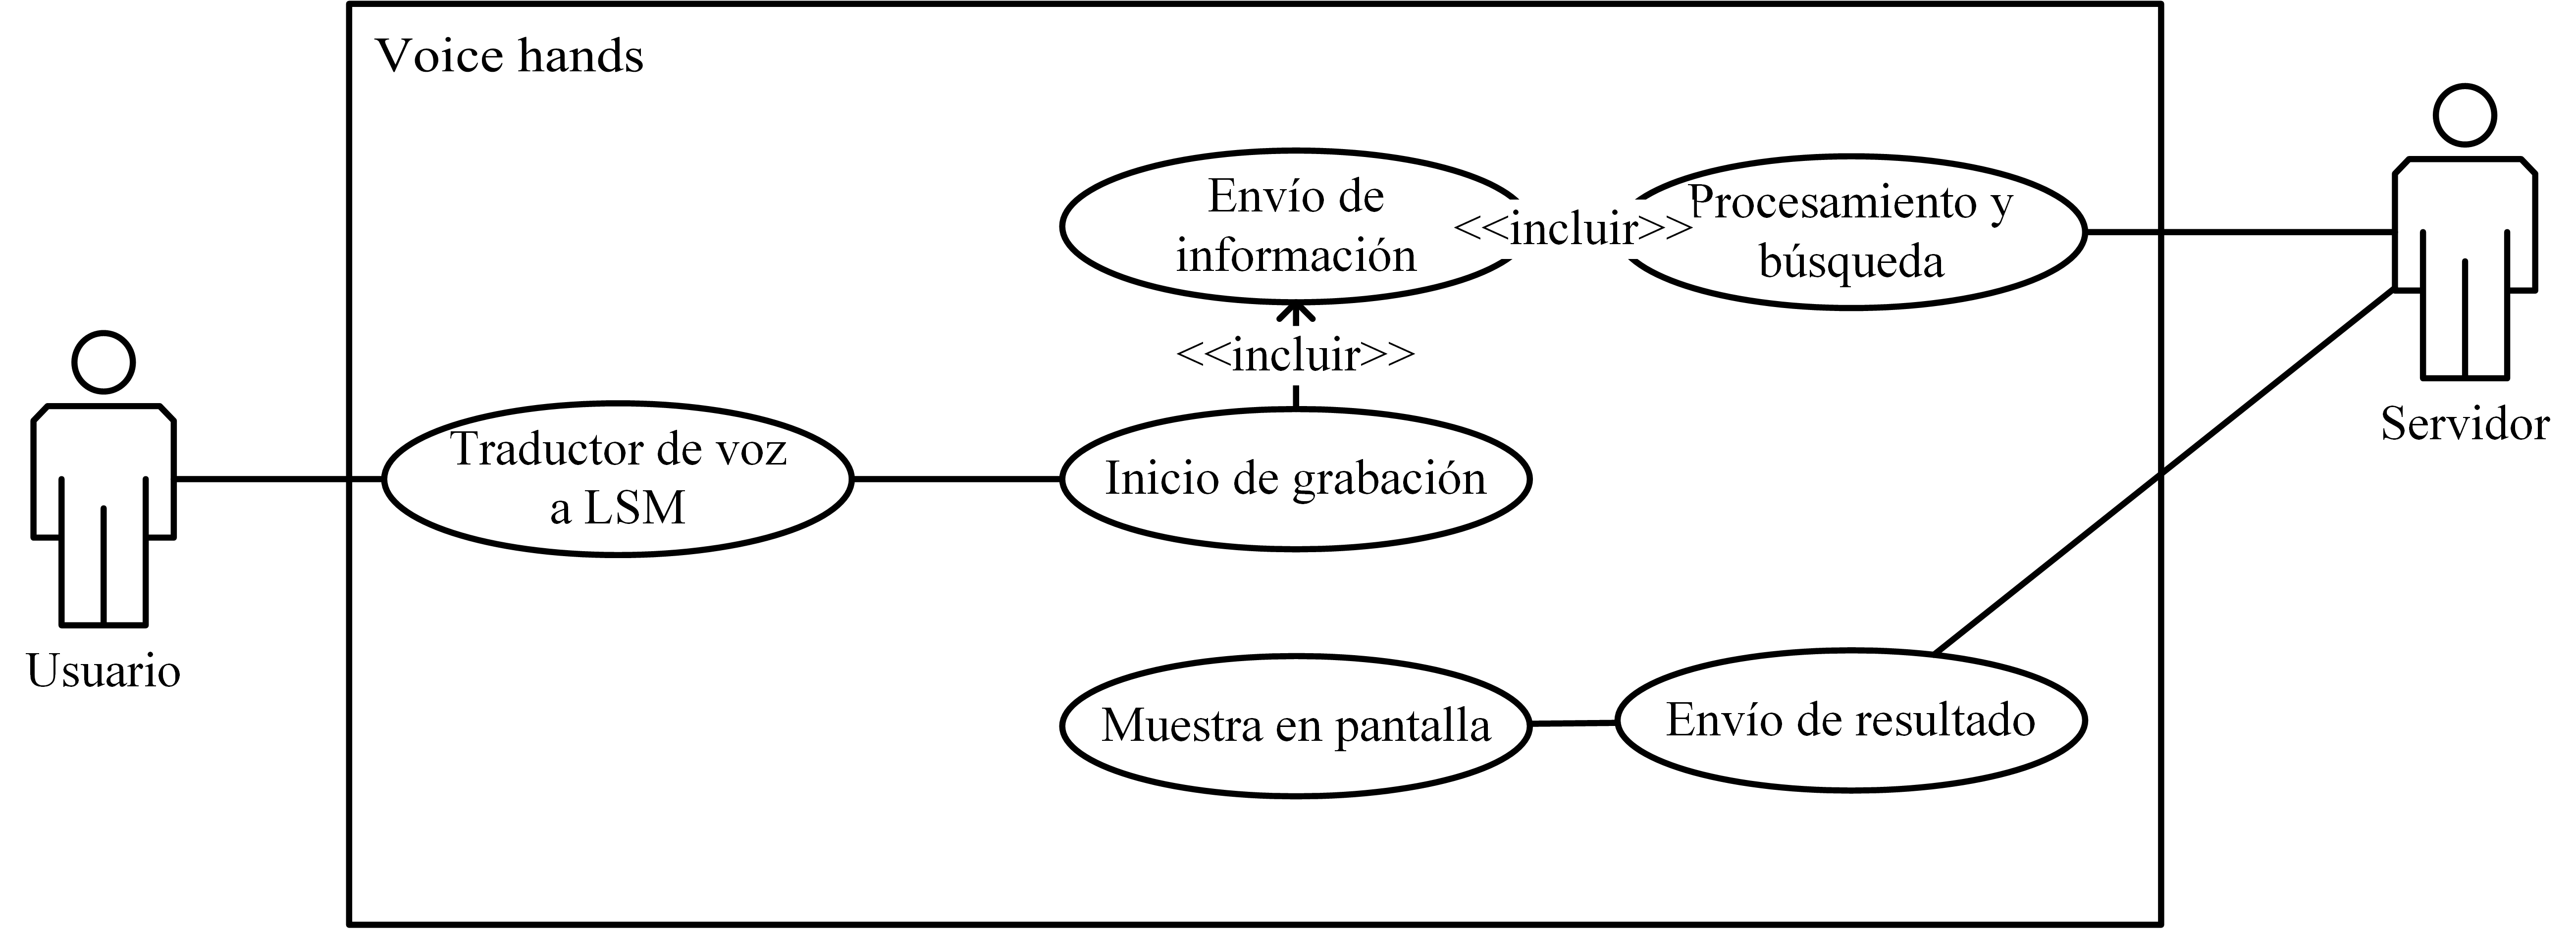
\includegraphics[width=0.8\linewidth]{figures/casoUsoVoz}
			\caption{Caso de uso \textit{``Traductor de voz''}}
			\label{fig:casoUsoVoz}
		\end{figure}
		
\paragraph{Síntesis de voz desde el teclado}\paragraph{}

En la Tabla \ref{tb:casoUsoSintesis} se muestra la especificación de la Figura \ref{fig:casoUsoSintesis} que corresponde al caso de uso de síntesis de voz en el cual, la persona que usa el LSM desea comunicarse con una persona que no lo usa.
		
\begin{table}[H]
\centering
\caption{Caso de uso \textit{``Síntesis de voz desde el teclado''}}
\label{tb:casoUsoSintesis}
\begin{tabular}{|l|l|}
\hline
\multicolumn{2}{|l|}{\cellcolor[HTML]{C0C0C0}Caso de uso: Síntesis de voz desde el teclado}                                                                                                                              \\ \hline
\multicolumn{2}{|l|}{Actor: Usuario, Aplicación móvil}                                                                                                                                                                   \\ \hline
\multicolumn{2}{|l|}{Descripción: Permite llevar a cabo la síntesis de voz del texto ingresado mediante el teclado}                                                                                                      \\ \hline
Curso normal                                                                                          & Alternativas                                                                                                     \\ \hline
\begin{tabular}[c]{@{}l@{}}1.	El usuario selecciona la función de \\ síntesis de voz\end{tabular}     &                                                                                                                  \\ \hline
\begin{tabular}[c]{@{}l@{}}2.	El usuario ingresa el texto en un campo \\ destinado.\end{tabular}      &                                                                                                                  \\ \hline
\begin{tabular}[c]{@{}l@{}}3.	Se da la opción de reproducir para \\ escuchar el mensaje.\end{tabular} & \begin{tabular}[c]{@{}l@{}}3.1.,Si el dispositivo no tiene conexión a \\ Internet se la hará saber.\end{tabular} \\ \hline
4.	Se reproduce el mensaje.                                                                           &                                                                                                                  \\ \hline
\end{tabular}
\end{table}

		\begin{figure}[H]
			\centering
			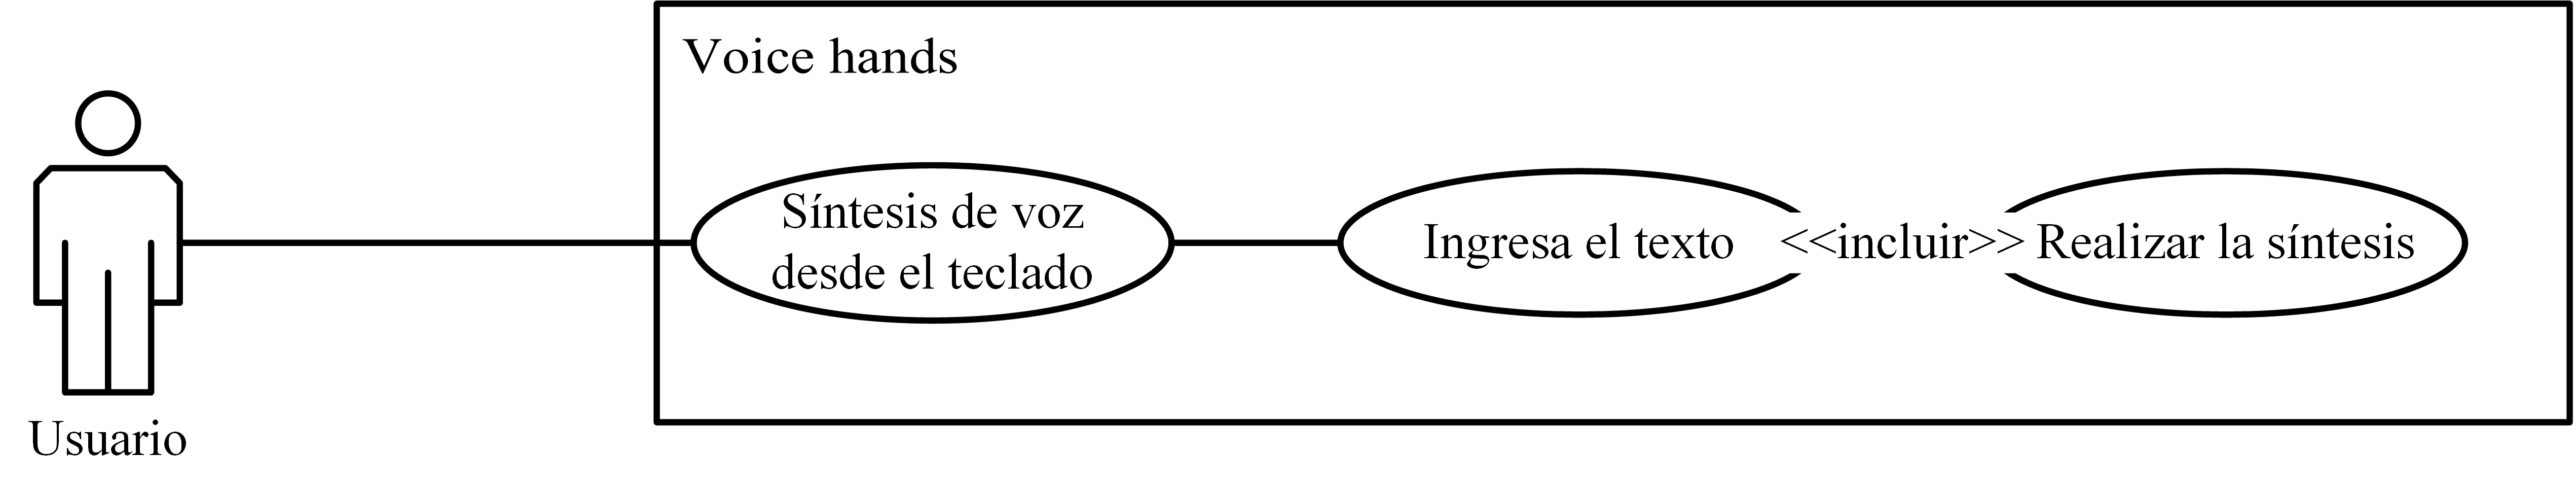
\includegraphics[width=0.8\linewidth]{figures/casoUsoSintesis}
			\caption{Caso de uso \textit{``Síntesis de voz desde el teclado''}}
			\label{fig:casoUsoSintesis}
		\end{figure}
		
\paragraph{Consulta de diccionario}\paragraph{}

En la Tabla \ref{tb:casoUsoDicc} se muestra la especificación de la Figura \ref{fig:casoUsoDicc} que corresponde al caso de uso de consulta de diccionario, en el que podemos encontrar vocabulario de diferentes categorías, así como las instrucciones para llevar a cabo la seña correspondiente.

% Please add the following required packages to your document preamble:
% \usepackage[table,xcdraw]{xcolor}
% If you use beamer only pass "xcolor=table" option, i.e. \documentclass[xcolor=table]{beamer}
\begin{table}[H]
\centering
\caption{Caso de uso \textit{``Consulta de diccionario''}}
\label{tb:casoUsoDicc}
\scalebox{0.9}{
\begin{tabular}{|l|l|}
\hline
\multicolumn{2}{|l|}{\cellcolor[HTML]{C0C0C0}Caso de uso: Consulta de diccionario}                                                                                                                                                           \\ \hline
\multicolumn{2}{|l|}{Actor: Usuario, Aplicación móvil, base de datos local.}                                                                                                                                                                 \\ \hline
\multicolumn{2}{|l|}{\begin{tabular}[c]{@{}l@{}}Descripción: Permite realizar la consulta de una palabra \\ obteniendo la seña e instrucciones para llevarla a cabo.\end{tabular}}                                                           \\ \hline
Curso normal                                                                                                 & Alternativas                                                                                                                  \\ \hline
\begin{tabular}[c]{@{}l@{}}1.   El usuario selecciona la función de consulta de\\  diccionario.\end{tabular} &                                                                                                                               \\ \hline
2.   Selecciona la categoría a consultar.                                                                    &                                                                                                                               \\ \hline
3.   Selecciona la palabra deseada.                                                                          & \begin{tabular}[c]{@{}l@{}}3.1.   Puede hacer uso del filtro de palabras\\ para encontrar más rápido la deseada.\end{tabular} \\ \hline
4.   Se muestra la información en pantalla.                                                                  &                                                                                                                               \\ \hline
\end{tabular}}
\end{table}

		\begin{figure}[H]
			\centering
			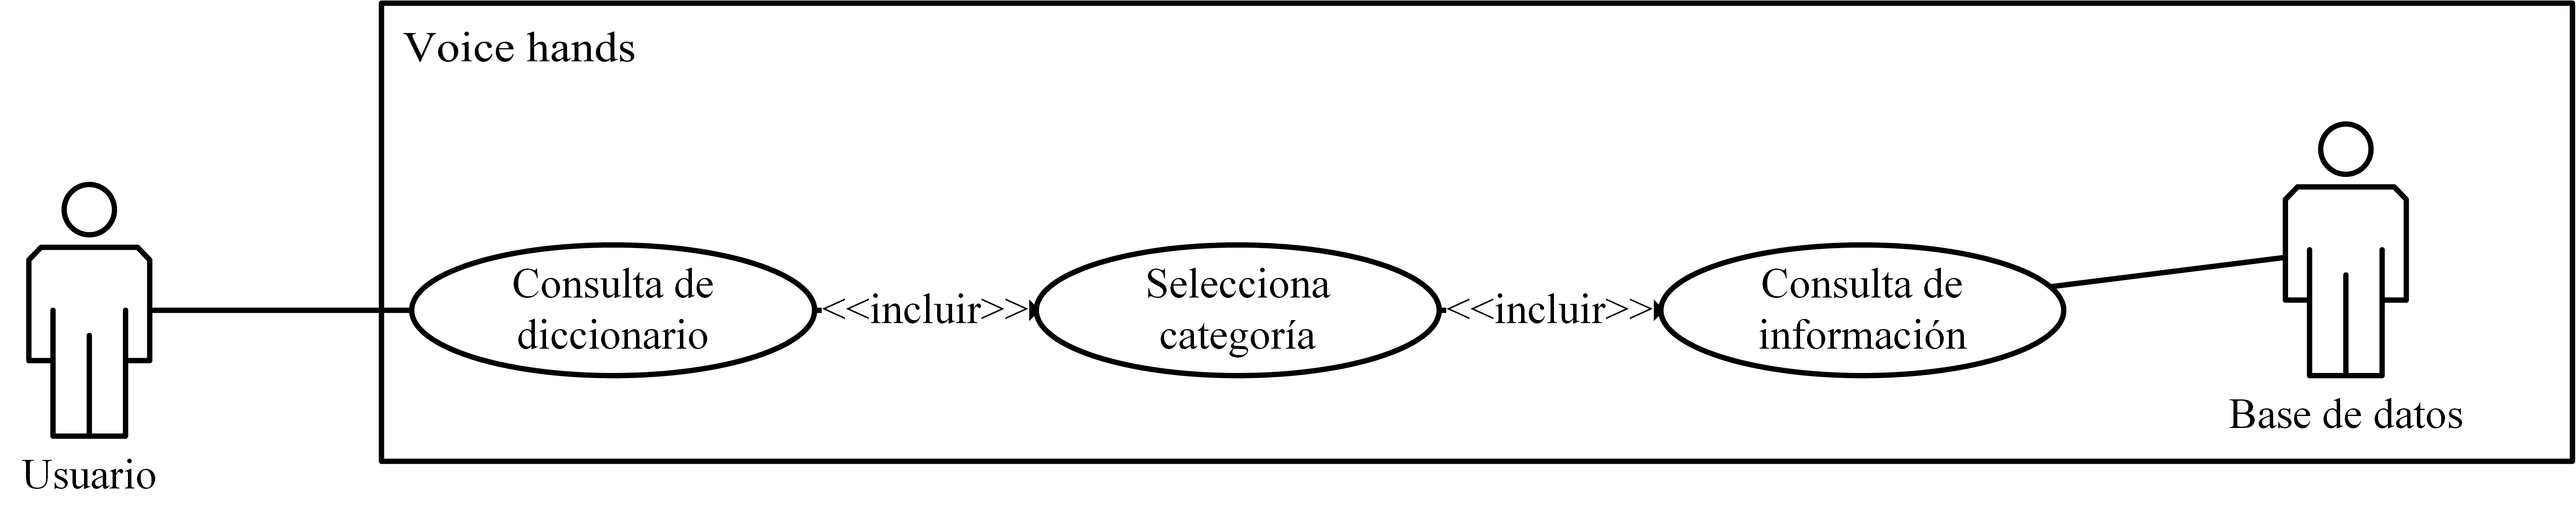
\includegraphics[width=0.8\linewidth]{figures/casoUsoDicc}
			\caption{Caso de uso \textit{``Consulta de diccionario''}}
			\label{fig:casoUsoDicc}
		\end{figure}
		
\subsubsection{Diagramas de actividades}

En la Figura \ref{fig:actVoz} se muestra la actividad del traductor de voz, así como las acciones que se deben llevar a cabo tanto por el usuario como por el móvil para obtener la traducción.


		\begin{figure}[H]
			\centering
			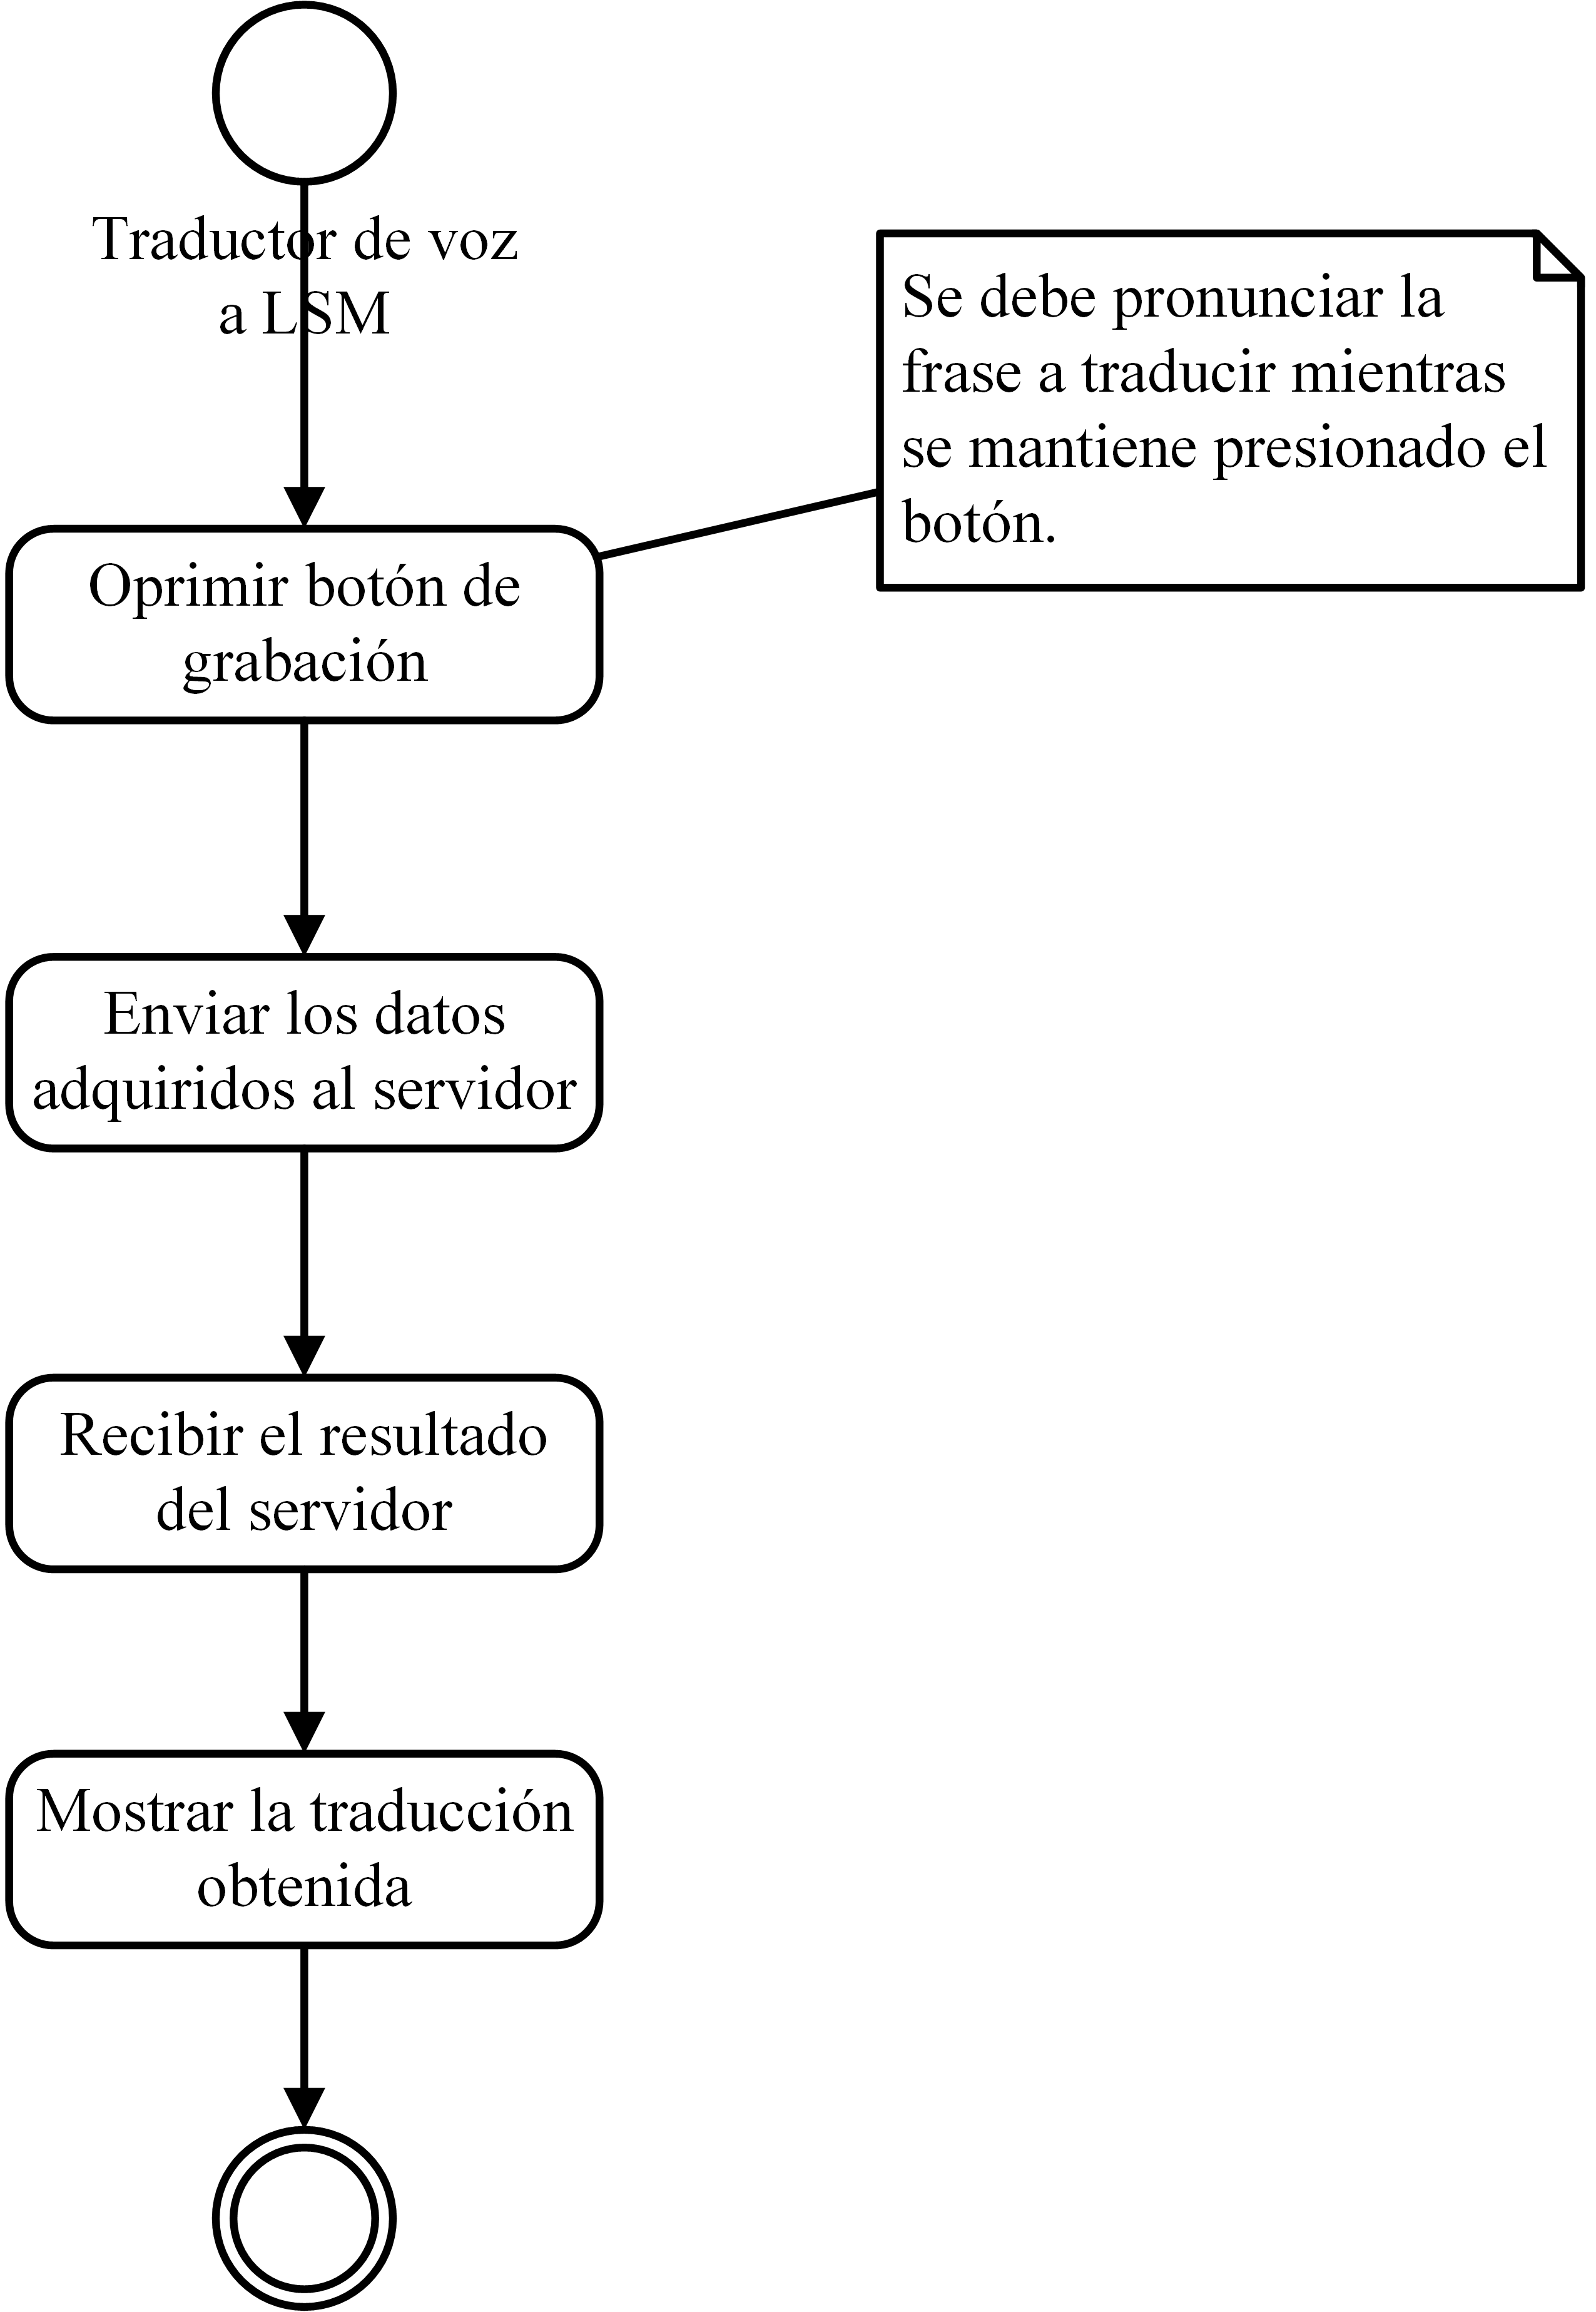
\includegraphics[width=0.5\linewidth]{figures/actVoz}
			\caption{Diagrama de actividad \textit{``Traductor de voz a LSM''}}
			\label{fig:actVoz}
		\end{figure}
		
En la Figura \ref{fig:actSintesis} se muestra el proceso a seguir para llevar a cabo la síntesis de voz mediante la entrada de texto

		\begin{figure}[H]
			\centering
			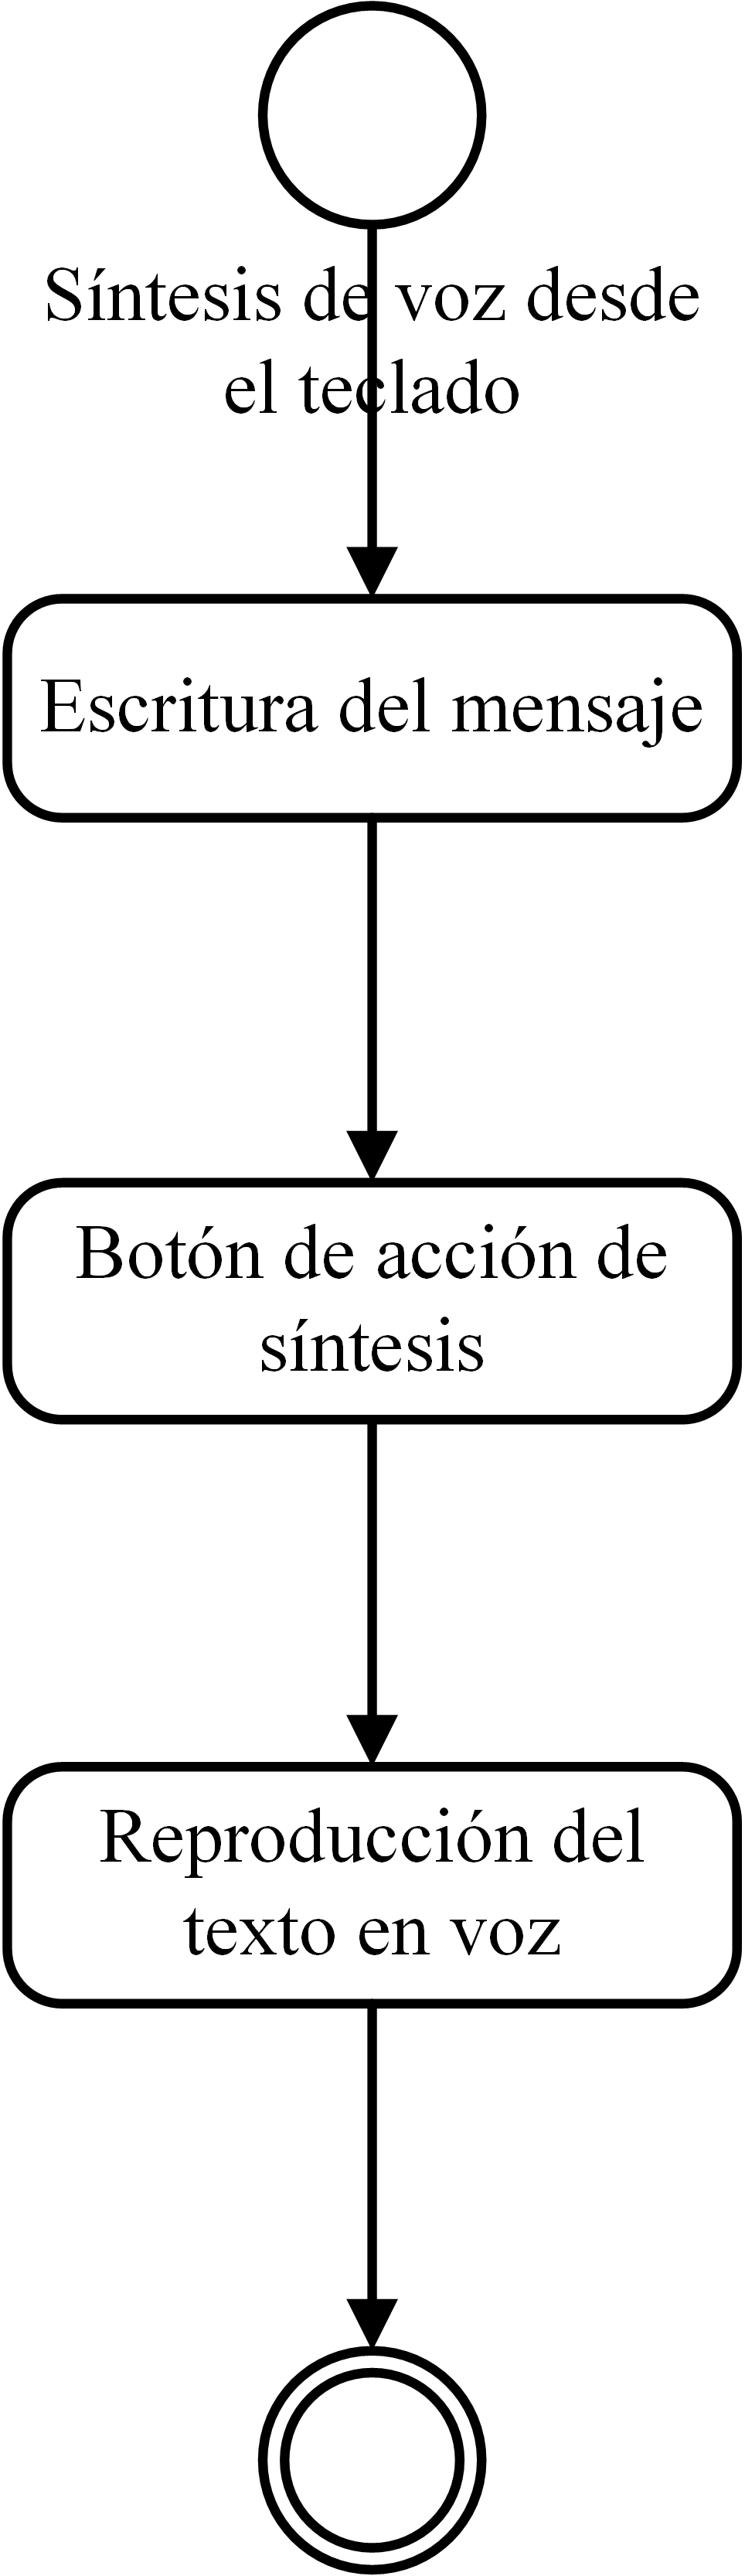
\includegraphics[width=0.2\linewidth]{figures/actSintesis}
			\caption{Diagrama de actividad \textit{``Síntesis de voz desde teclado''}}
			\label{fig:actSintesis}
		\end{figure}
		
En la Figura \ref{fig:actDicc} se muestra la acción de consultar el diccionario y el flujo de la consulta dependiendo de si se usa o no los filtros disponibles.		

		\begin{figure}[H]
			\centering
			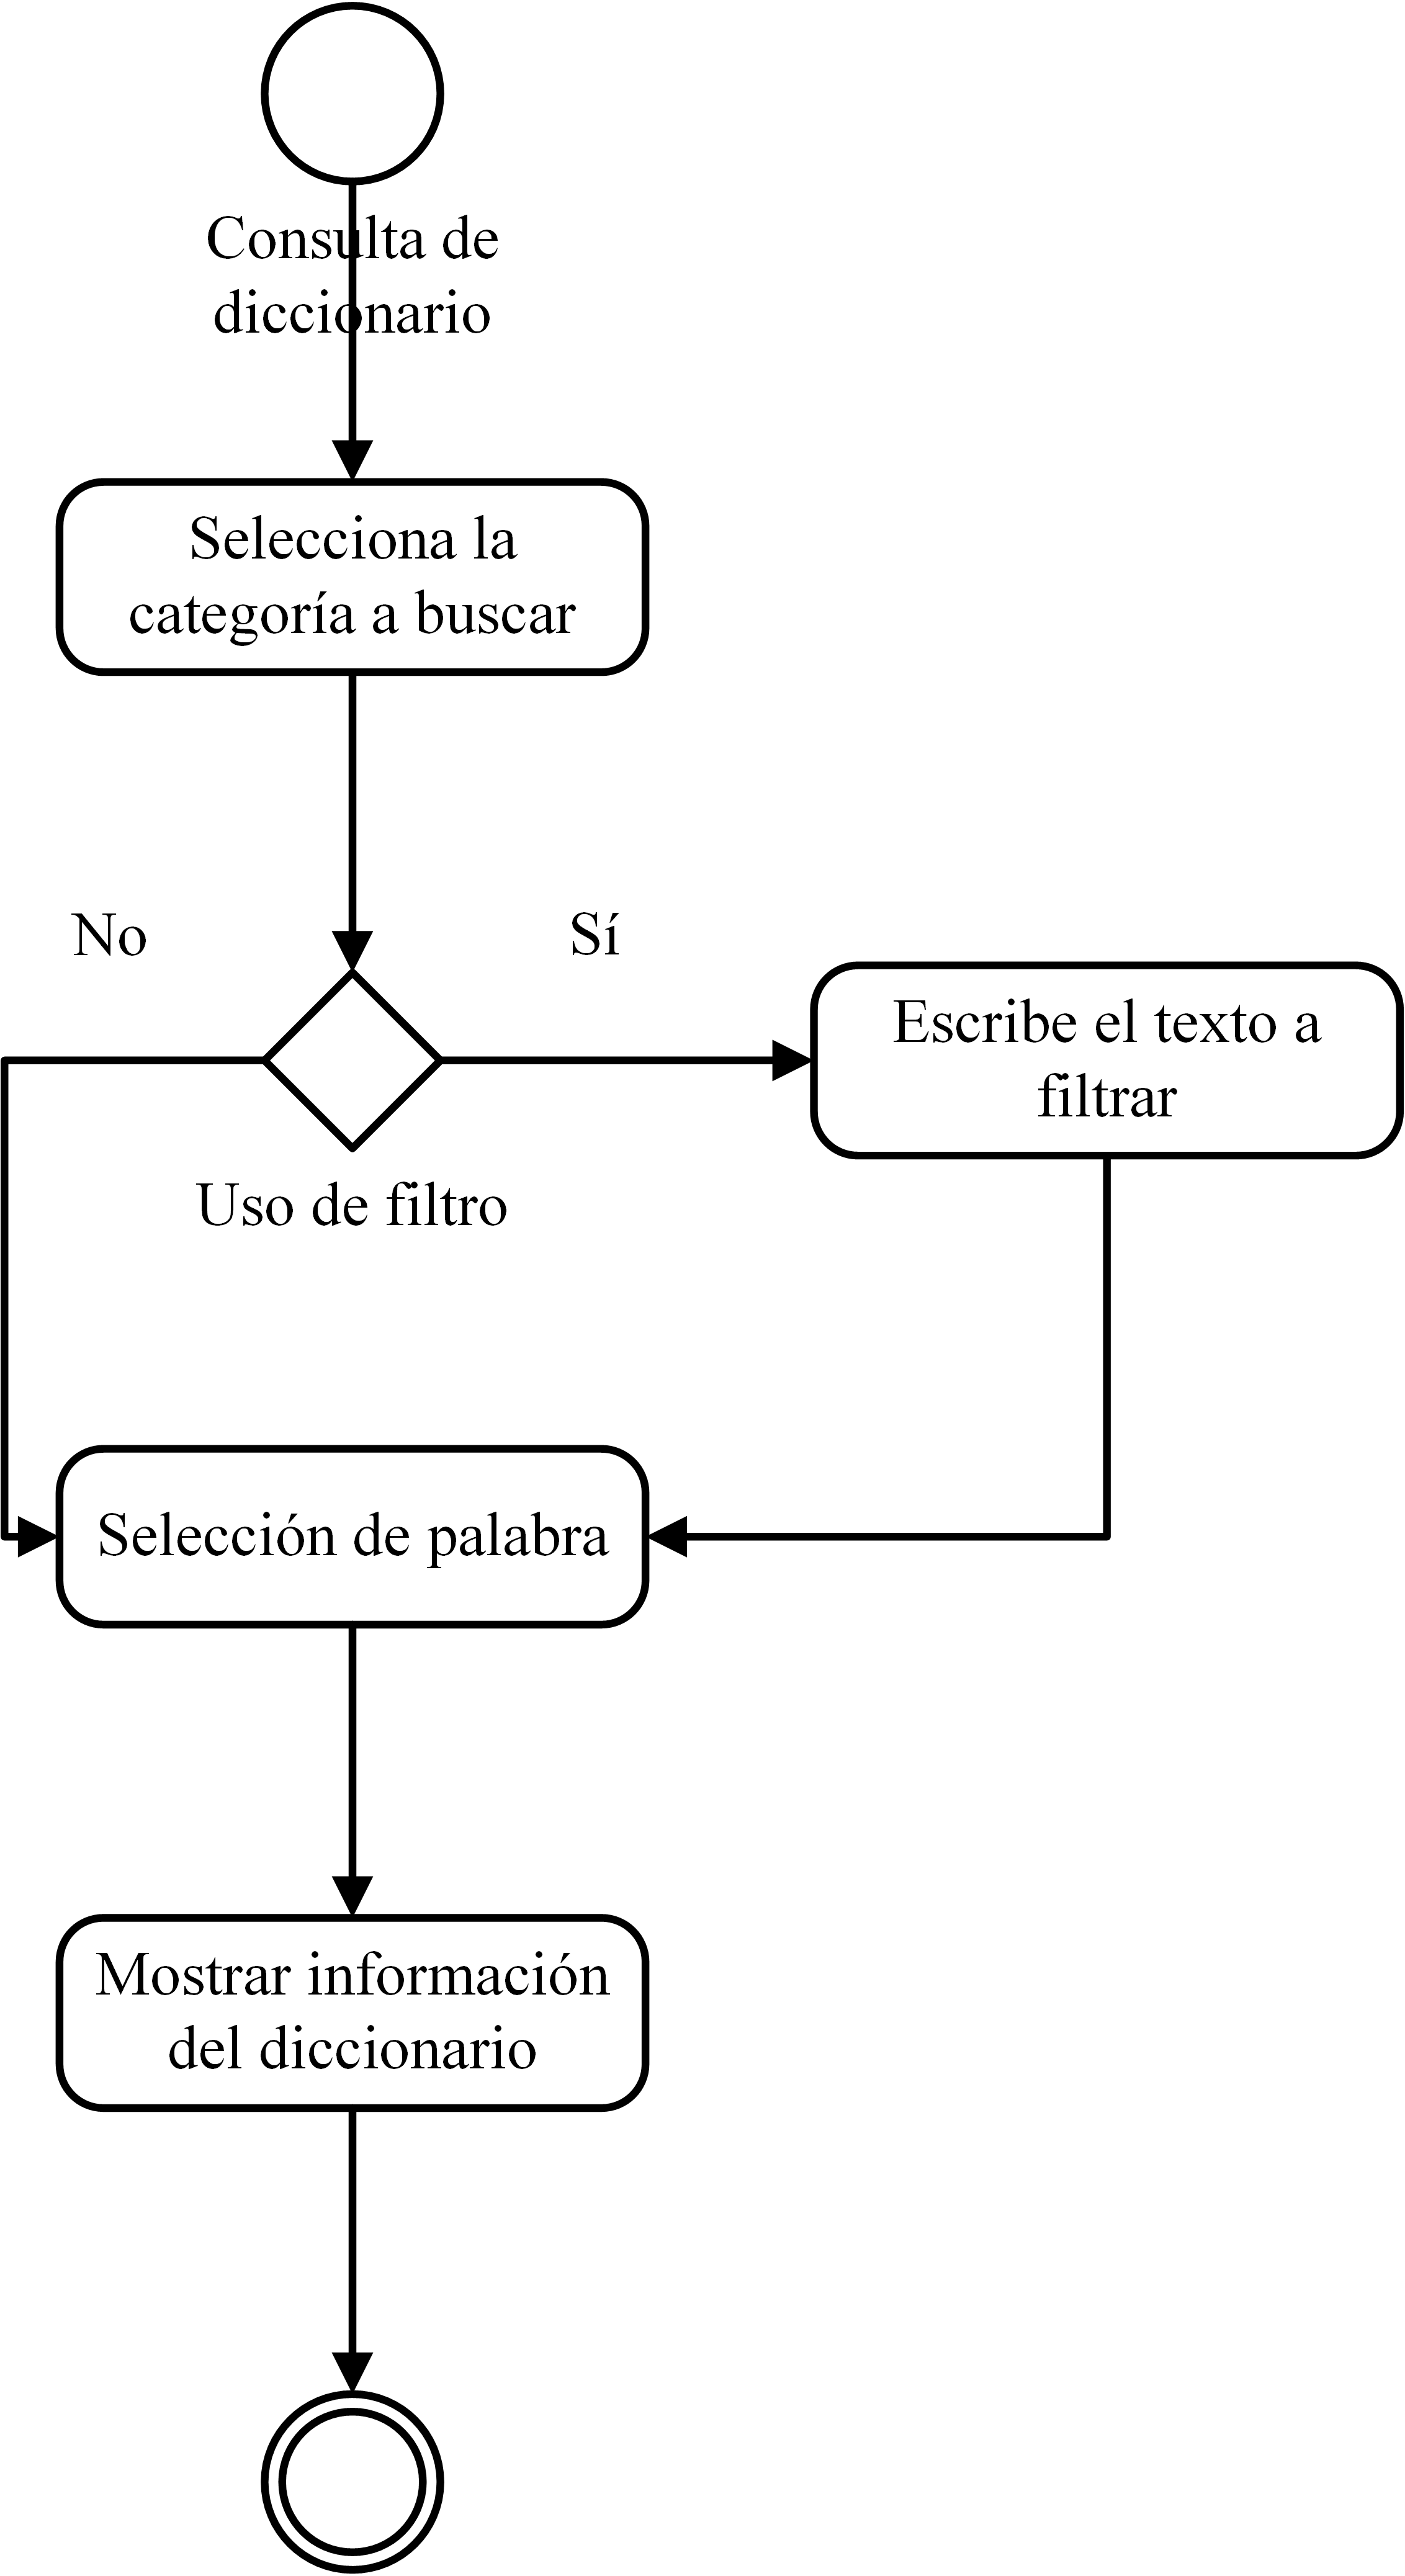
\includegraphics[width=0.5\linewidth]{figures/actDicc}
			\caption{Diagrama de actividad \textit{``Consulta de diccionario''}}
			\label{fig:actDicc}
		\end{figure}
		
\subsubsection{Diagramas de secuencia}

En los siguientes diagramas se muestra la secuencia de actividades a llevar a cabo para realizar las 3 tareas planteadas.

En la Figura \ref{fig:secVoz} se muestra la secuencia y la intervención de cada elemento del sistema para llevar a cabo la adquisición de voz y su respectiva traducción.

		\begin{figure}[H]
			\centering
			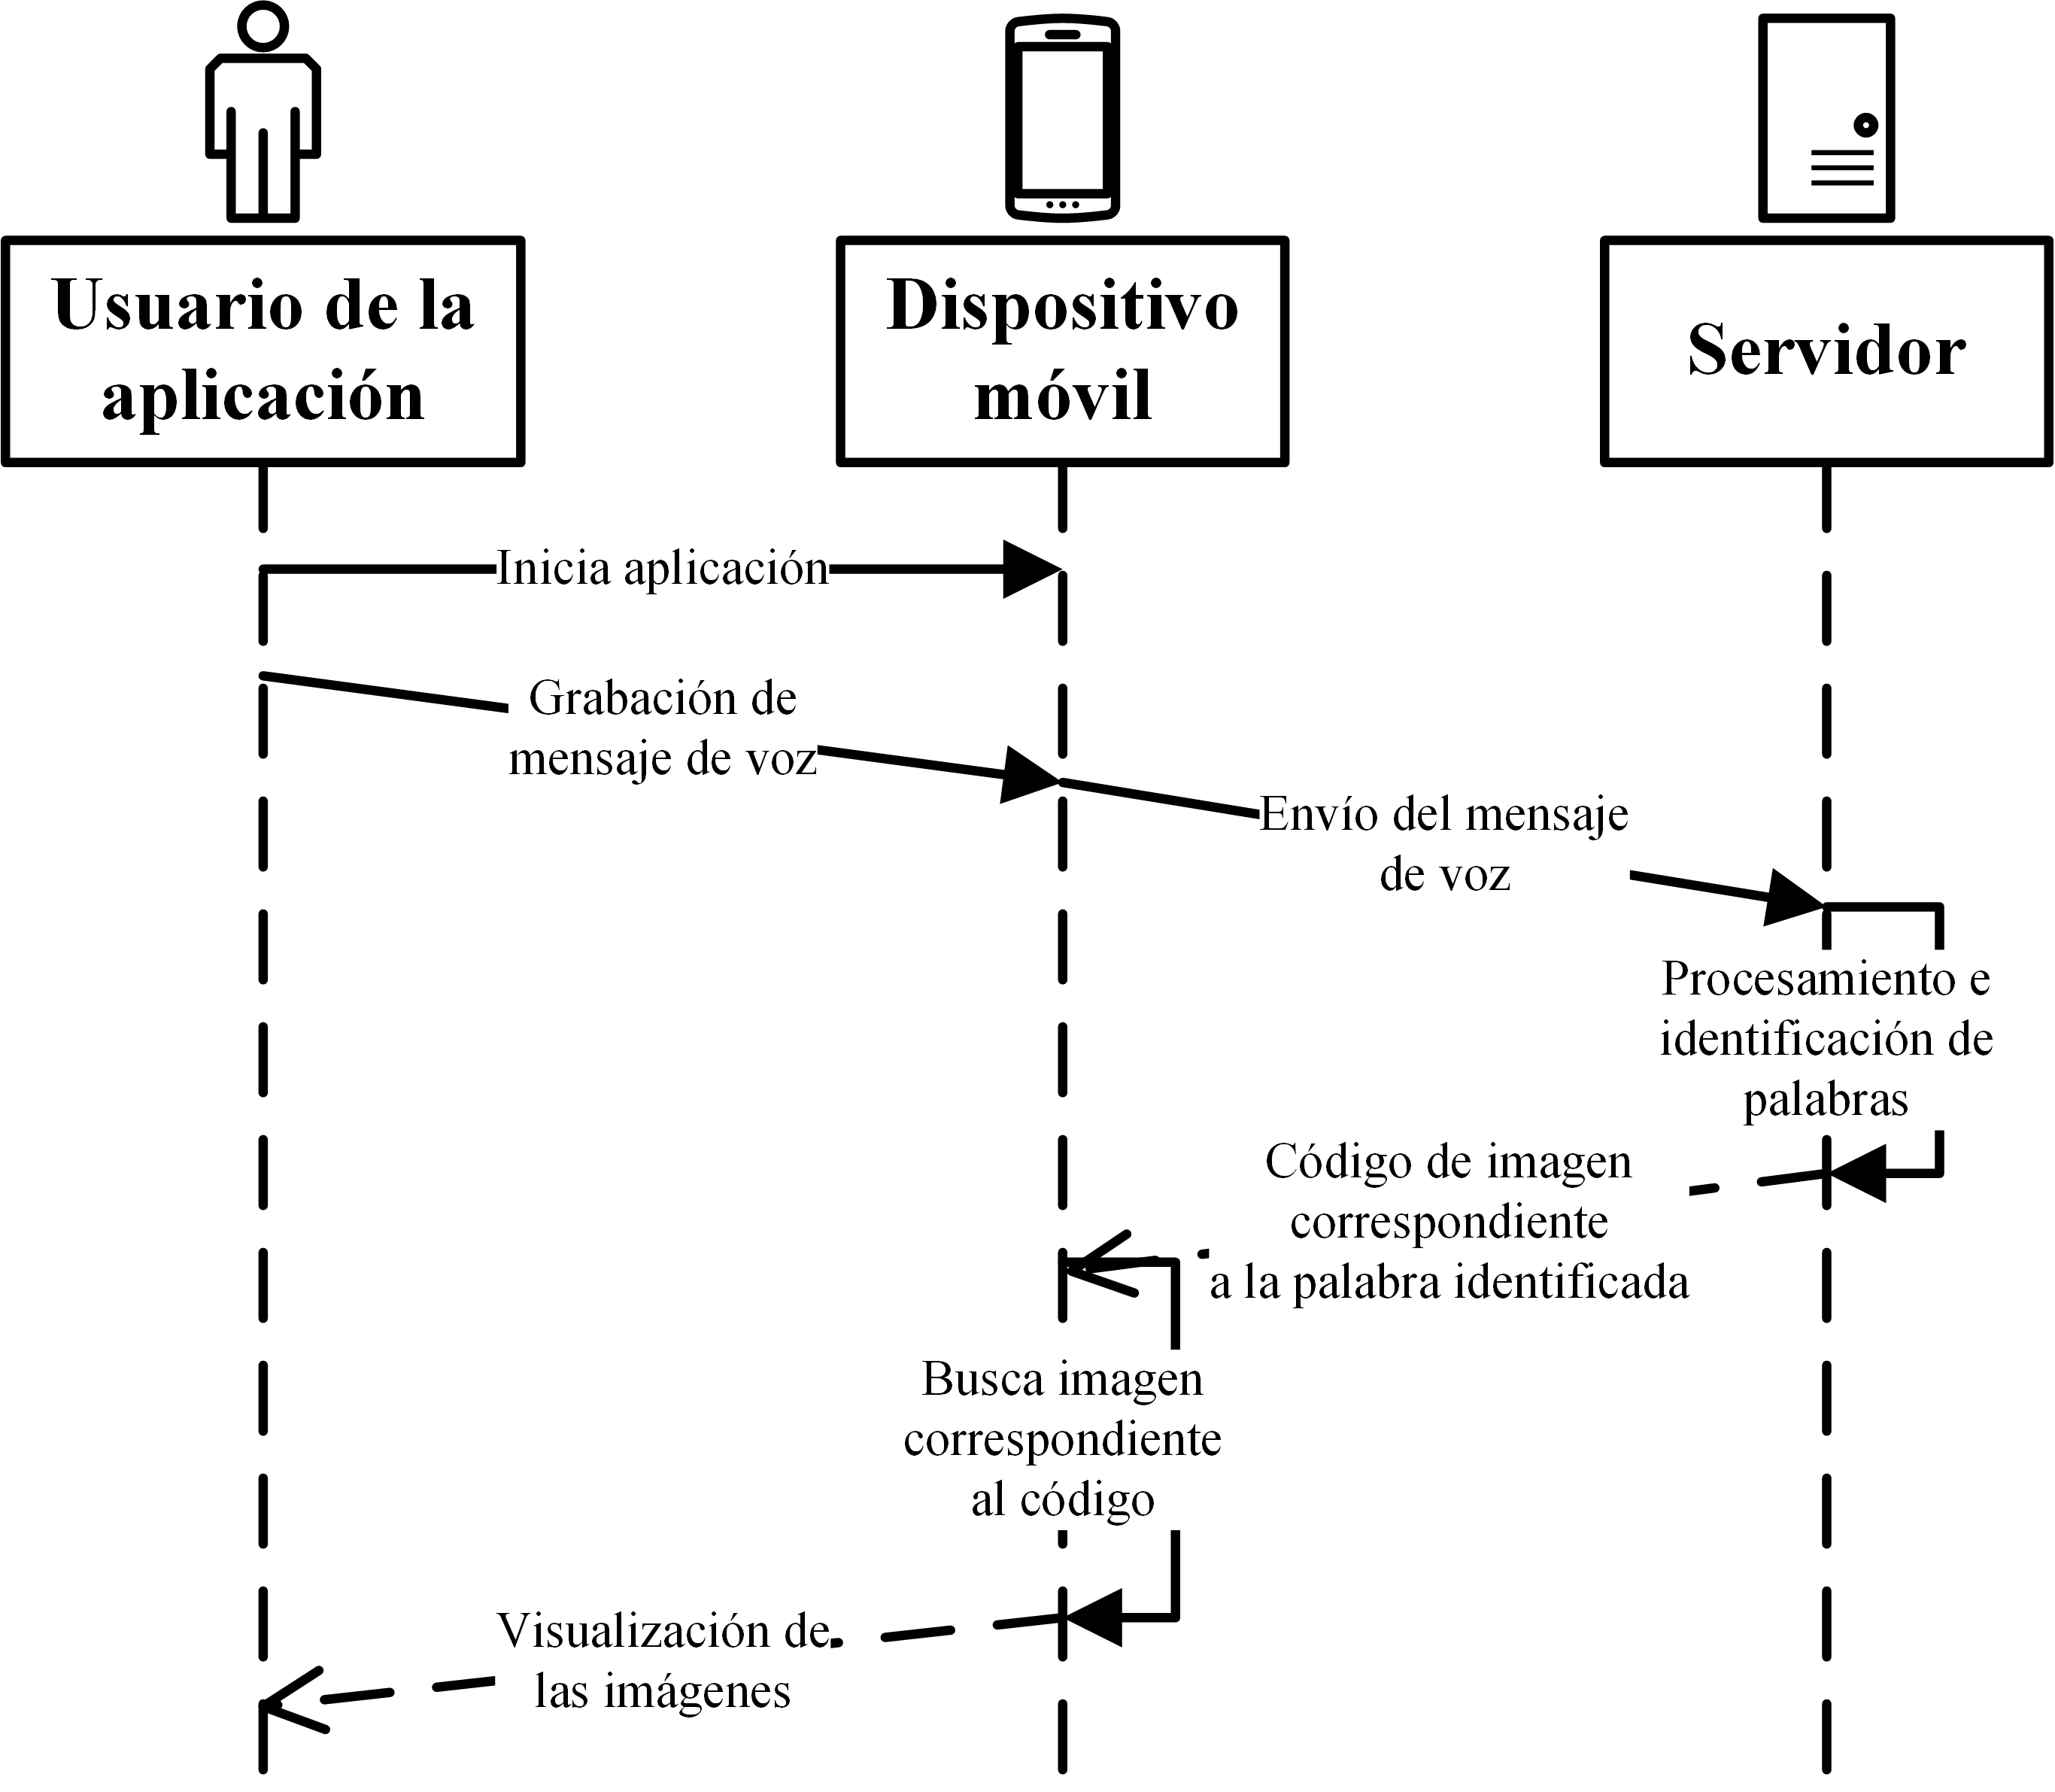
\includegraphics[width=0.7\linewidth]{figures/secuenciaVoz}
			\caption{Diagrama de secuencia \textit{``Traductor de voz a LSM''}}
			\label{fig:secVoz}
		\end{figure}
		
En la Figura \ref{fig:secSintesis} se muestra el diagrama de secuencia que muestra la interacción entre el actor y el dispositivo móvil para llevar a cabo la síntesis de voz del mensaje a transmitir.

		\begin{figure}[H]
			\centering
			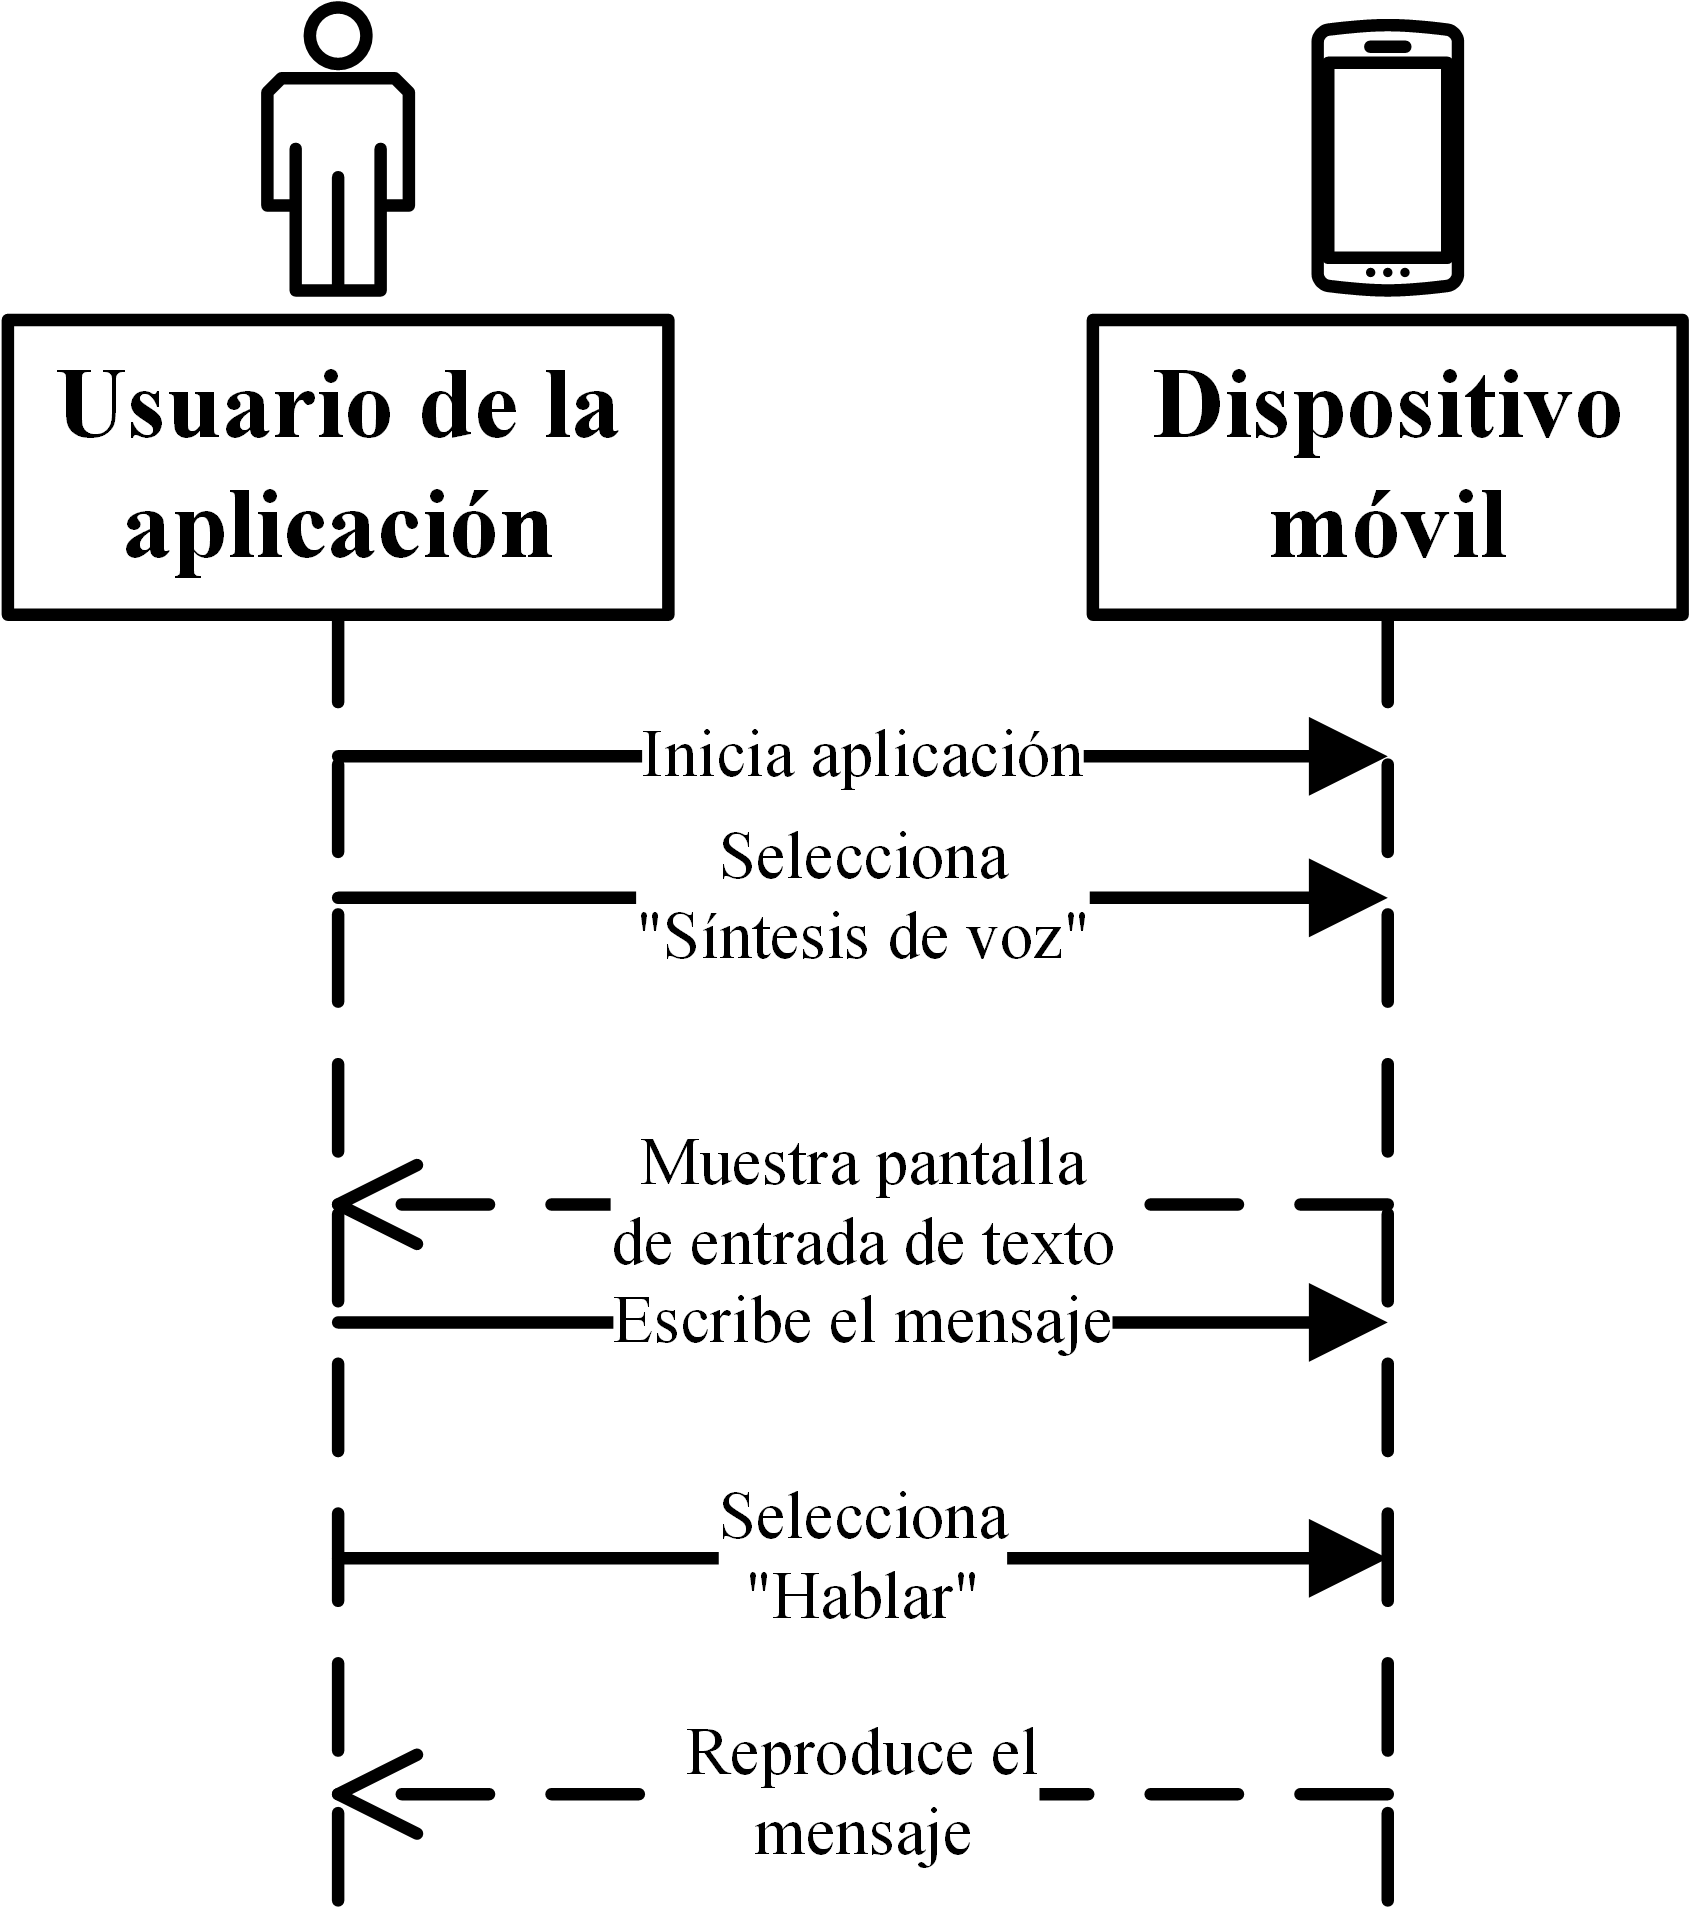
\includegraphics[width=0.5\linewidth]{figures/secuenciaSintesis}
			\caption{Diagrama de secuencia \textit{``Síntesis de voz desde teclado''}}
			\label{fig:secSintesis}
		\end{figure}		
		
Finalmente en la Figura \ref{fig:secDiccionario} se muestra la interacción entre el actor y el dispositivo móvil, con las acciones a realizar para obtener la descripción de la seña de determinada palabra.

		\begin{figure}[H]
			\centering
			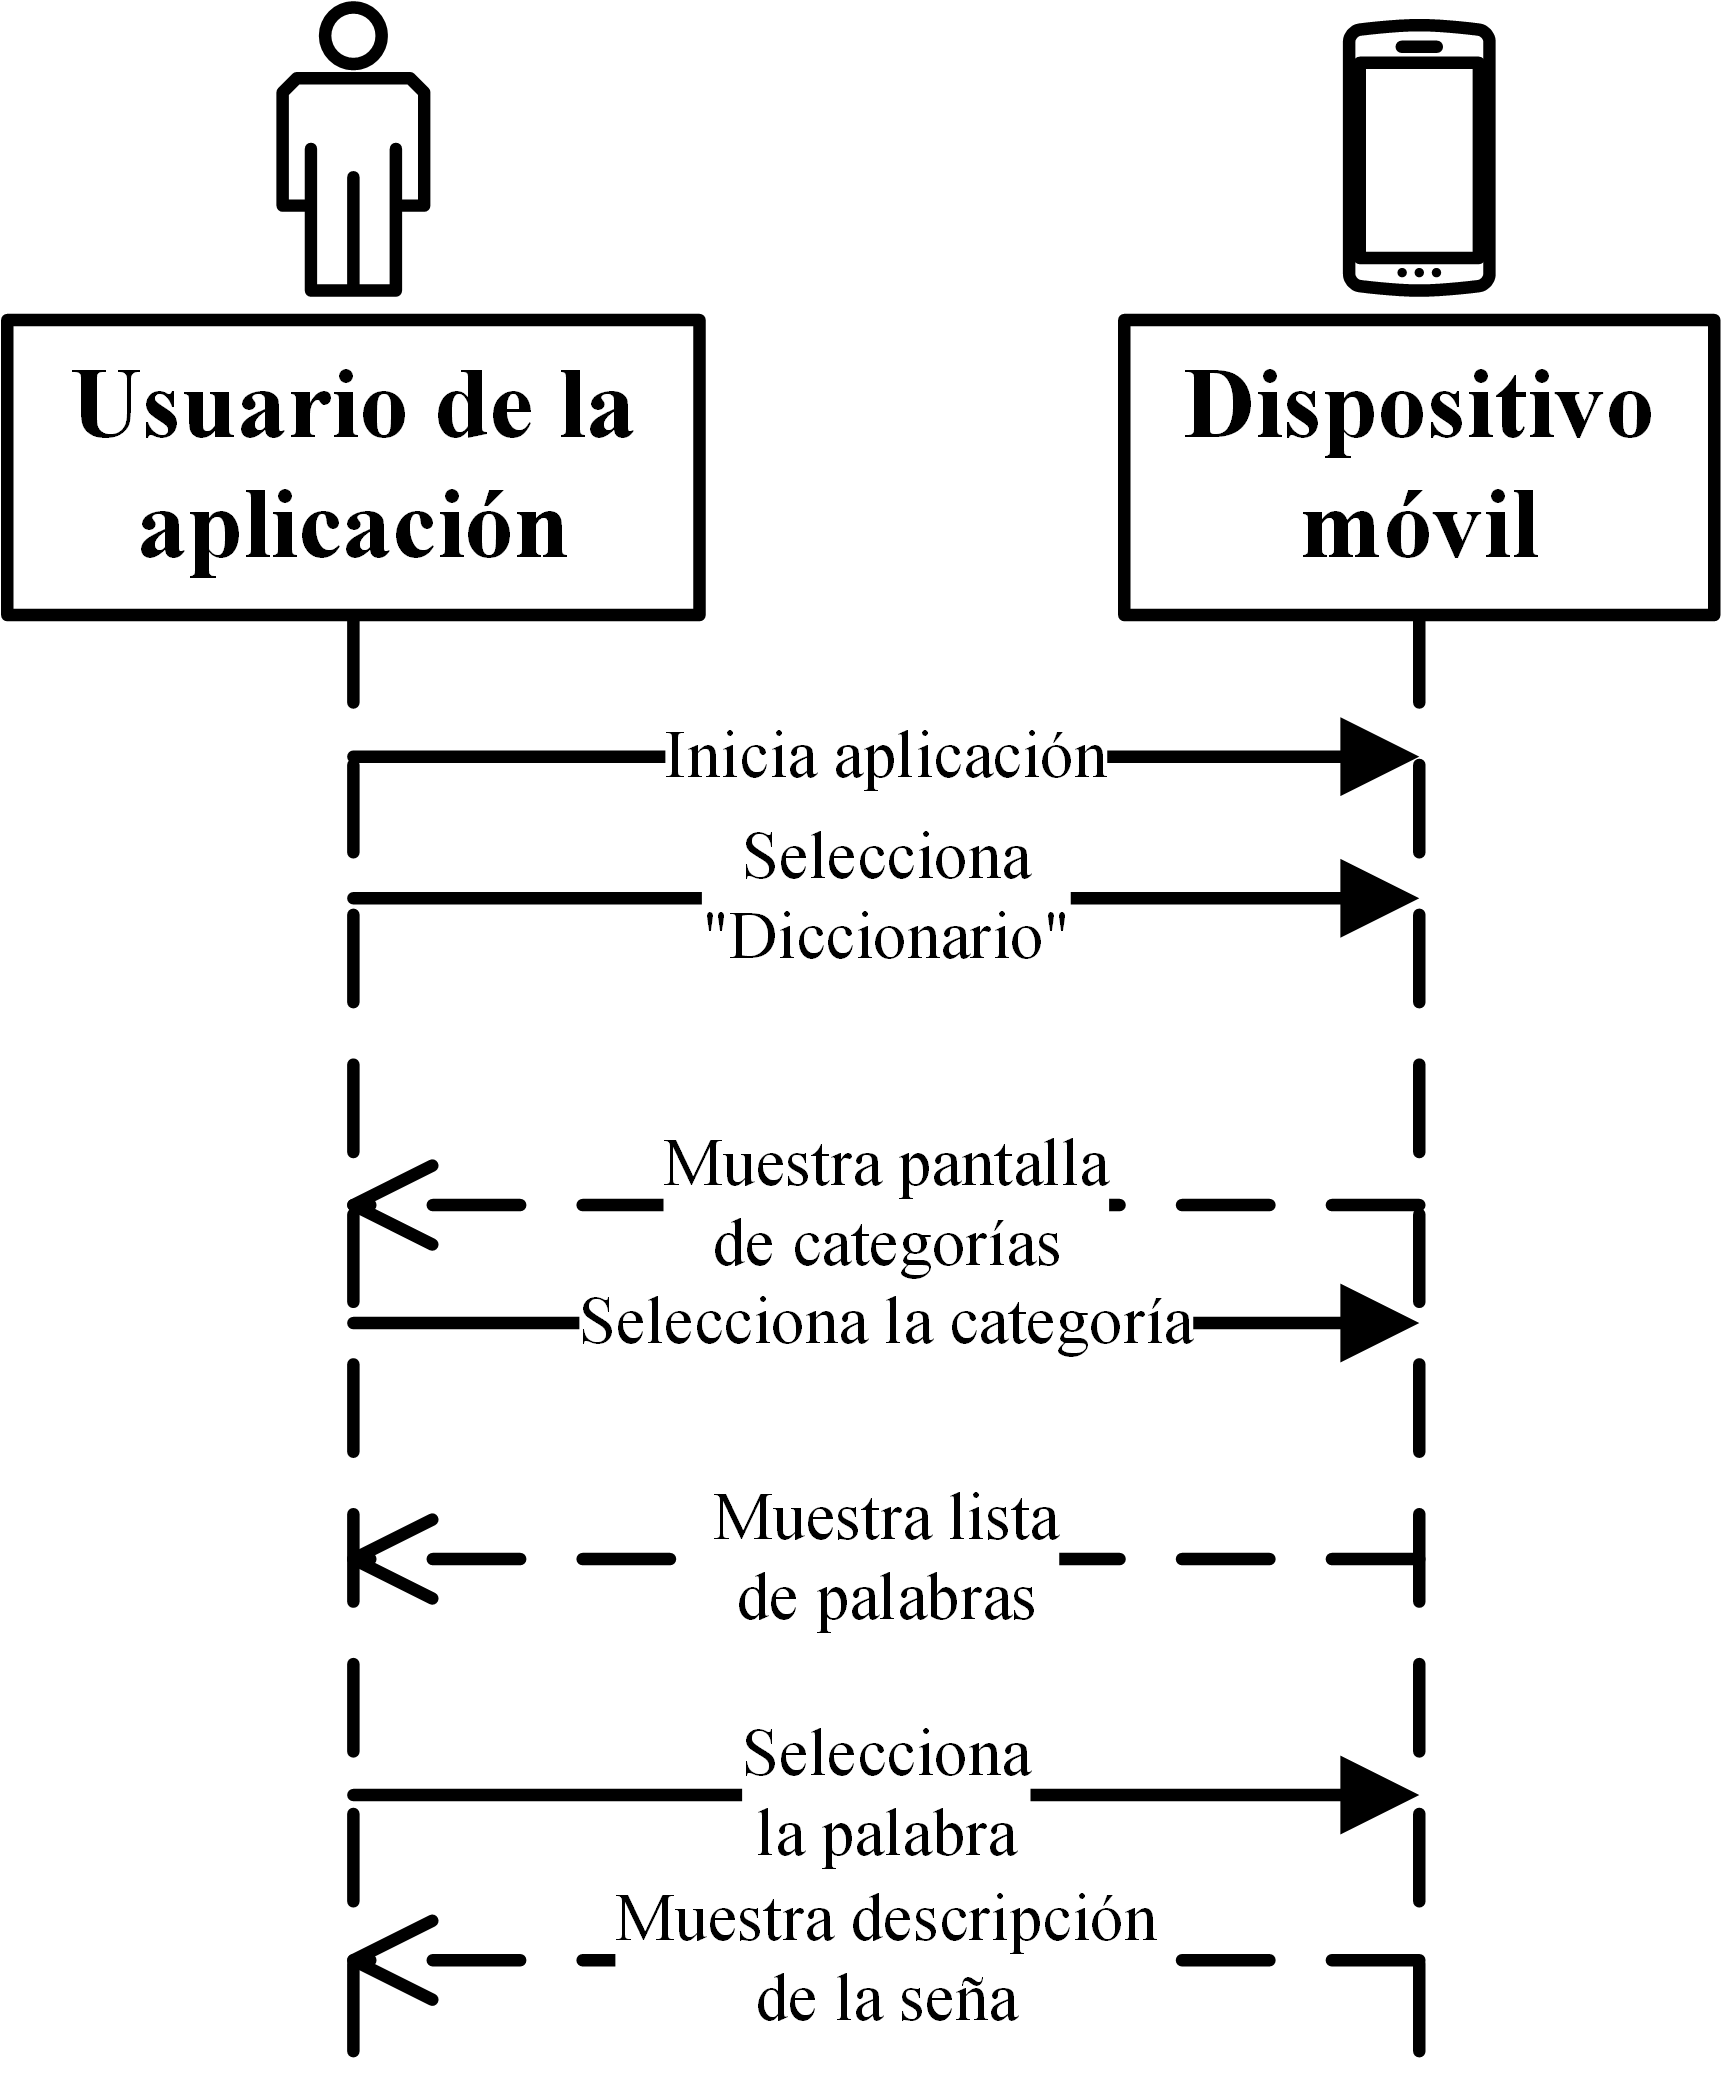
\includegraphics[width=0.5\linewidth]{figures/secuenciaDiccionario}
			\caption{Diagrama de secuencia \textit{``Consulta de diccionario''}}
			\label{fig:secDiccionario}
		\end{figure}		
		
\subsubsection{Base de datos}

La base de datos a implementar básicamente será una tabla la cual contendrá la palabra un código asociado, este código identificará a la imagen que debe ser presentada, el código será enviado al móvil el cual ya contiene todas las imágenes que corresponden a las palabras. En la Figura \ref{fig:database} se muestra la tabla de la base de datos a implementar.

		\begin{figure}[H]
			\centering
			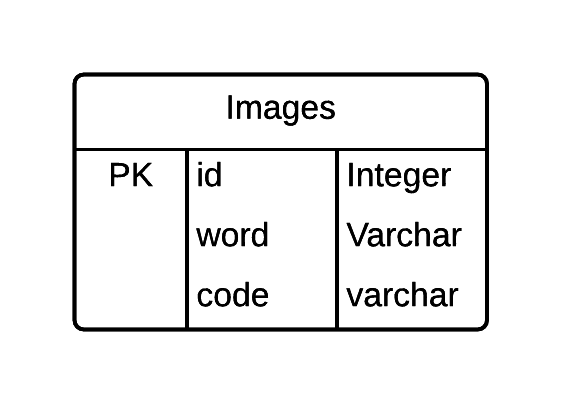
\includegraphics[width=0.5\linewidth]{figures/database}
			\caption{Base de datos a implementar}
			\label{fig:database}
		\end{figure}		

\subsubsection{Pantallas de la aplicación}

%\begin{multicols}{2} 

\begin{figure}[H]
	\centering
	
\includegraphics[scale = 0.2]{figures/app01}
	\caption{Aplicación: Splash Screen}
	\label{fig:app01}
\end{figure}

La primera pantalla de la aplicación es un Splash Screen en la cual se muestra en nombre e icono durante 3 segundos.

\begin{figure}[H]
	\centering
	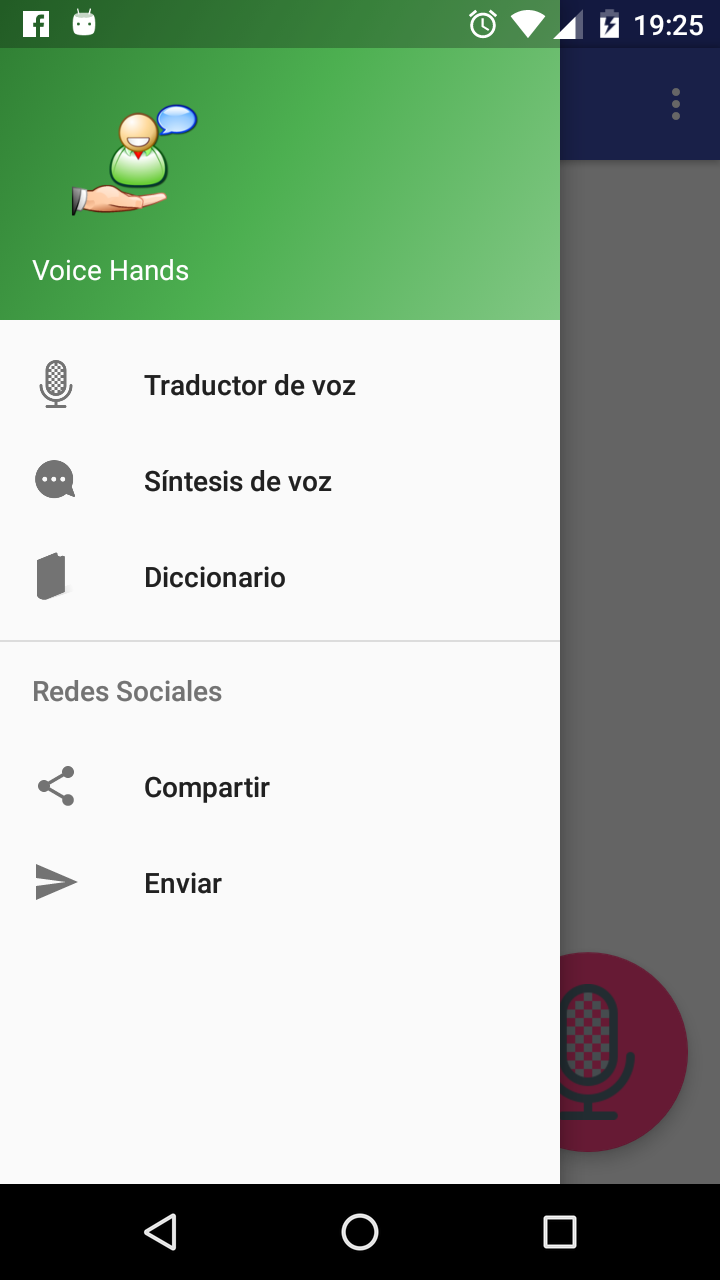
\includegraphics[scale = 0.2]{figures/app02}
	\caption{Aplicación: Menú lateral}
	\label{fig:app03}
\end{figure}

La aplicación cuenta con un menú lateral que nos mostrará las tres principales actividades, y mediante las cuales podremos acceder.

\begin{figure}[H]
	\centering
	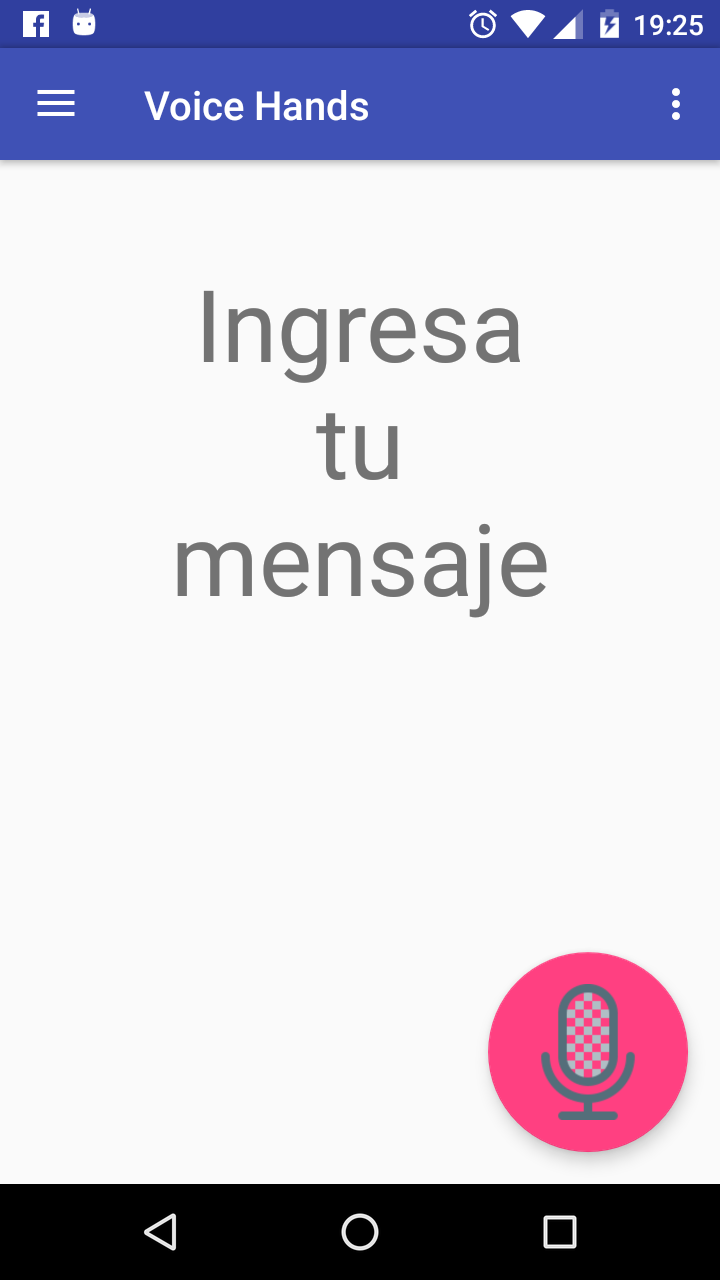
\includegraphics[scale = 0.2]{figures/app03}
	\caption{Aplicación: Pantalla principal}
	\label{fig:app02}
\end{figure}

La pantalla principal corresponde a la sección de traductor de voz a LSM.

\begin{figure}[H]
	\centering
	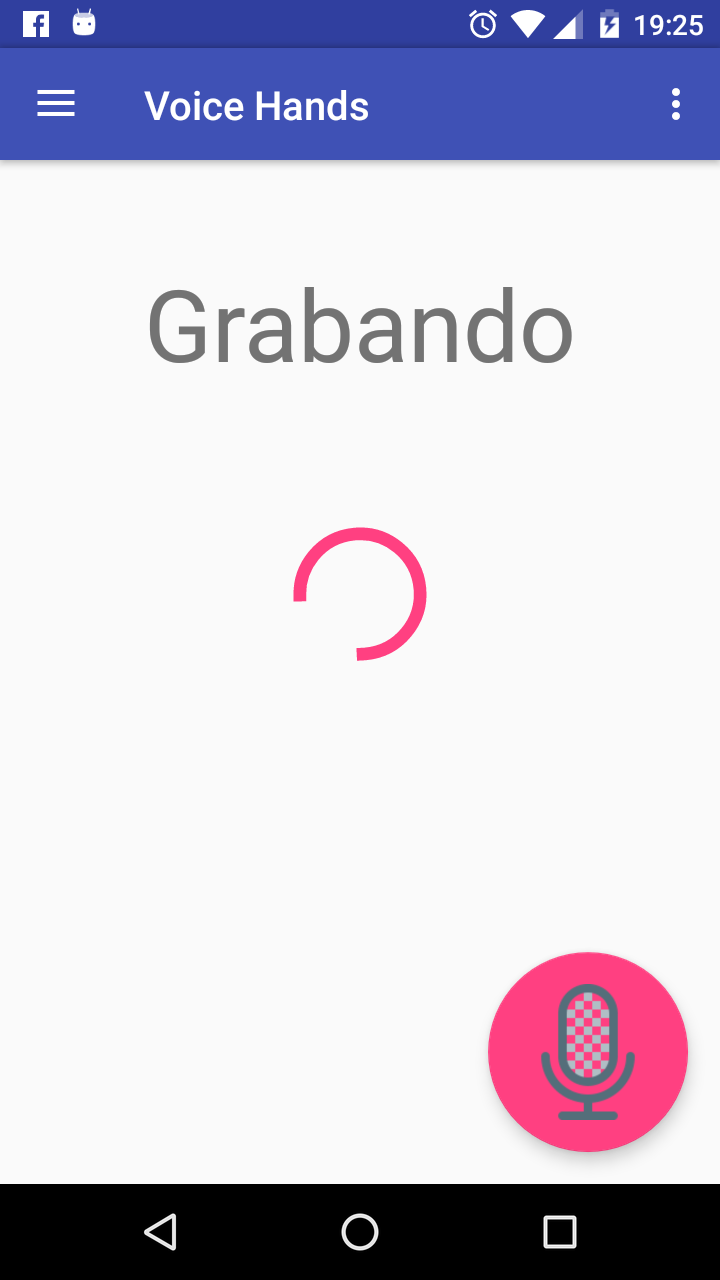
\includegraphics[scale = 0.2]{figures/app04}
	\caption{Aplicación: Grabación de voz}
	\label{fig:app04}
\end{figure}

Al seleccionar el traductor de voz a LSM contaremos con un botón flotante que es el que nos permitirá grabar la frase que queremos traducir, y se nos mostrará una barra de progreso lo que nos indica el tiempo restante para completar la grabación.

\begin{figure}[H]
	\centering
	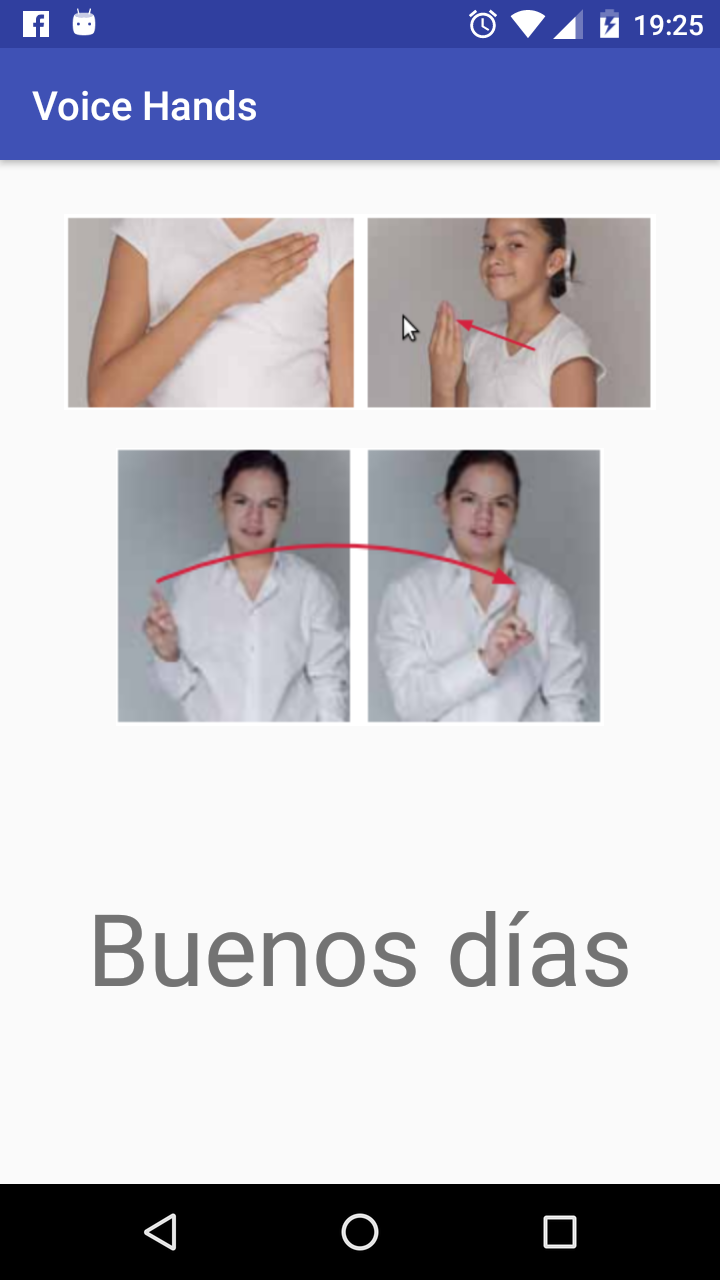
\includegraphics[scale = 0.2]{figures/app05}
	\caption{Aplicación: Traducción}
	\label{fig:app05}
\end{figure}

Una vez hecho esto, el sistema se encarga de enviar y recibir la información, para que después nos muestre en pantalla la imagen o imágenes resultantes de la traducción.

\begin{figure}[H]
	\centering
	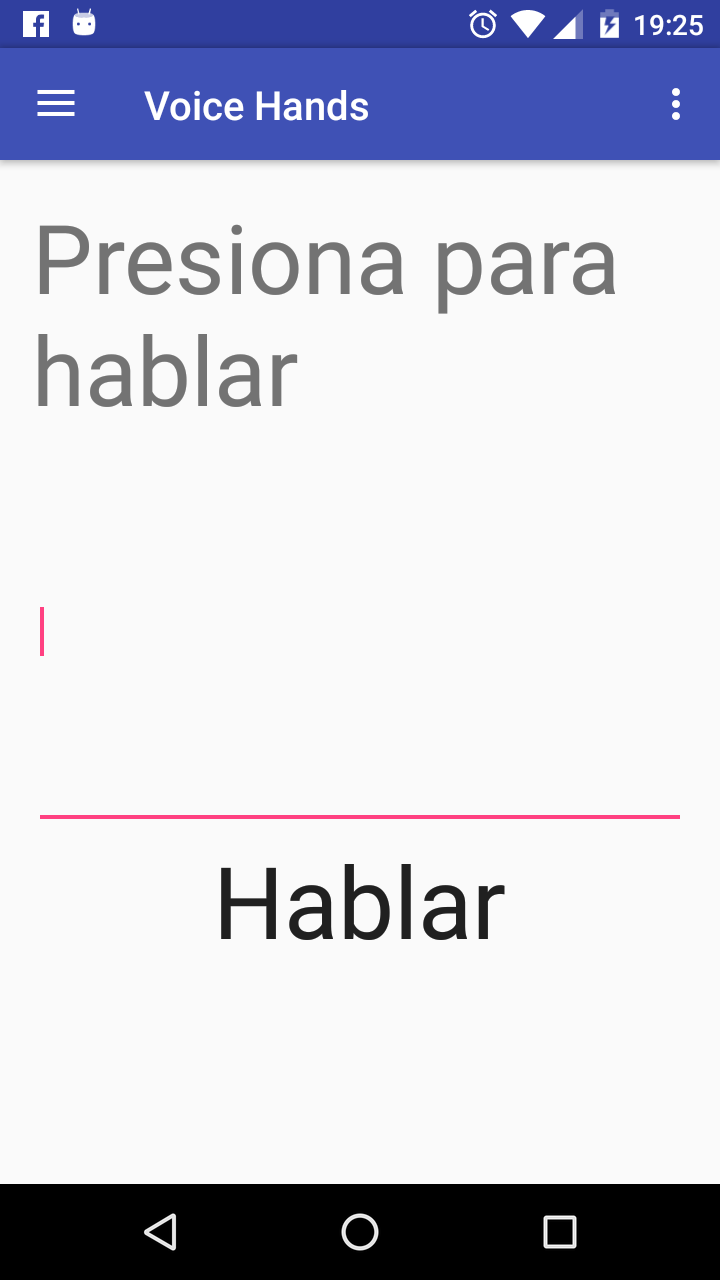
\includegraphics[scale = 0.2]{figures/app06}
	\caption{Aplicación: Campo de escritura para síntesis}
	\label{fig:app06}
\end{figure}

Si seleccionamos la segunda opción del menú lateral o la síntesis de voz, la aplicación nos mostrará esta actividad, en la cual tan sólo debemos ingresar el texto en el cuadro y al finalizar presionamos el botón pronunciar para que se realice la síntesis de voz.

\begin{figure}[H]
	\centering
	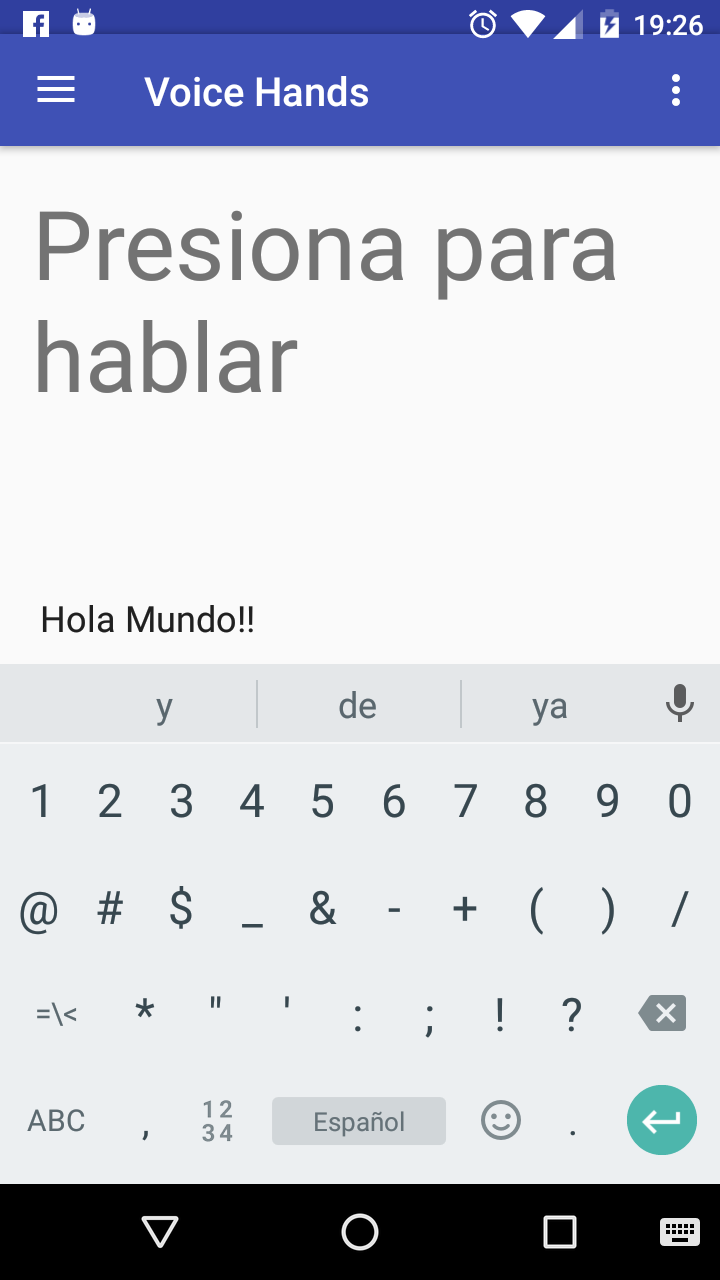
\includegraphics[scale = 0.2]{figures/app07}
	\caption{Aplicación: Entrada de texto}
	\label{fig:app07}
\end{figure}

En esta pantalla vemos cómo se muestra el teclado y se realiza la entrada de texto.

\begin{figure}[H]
	\centering
	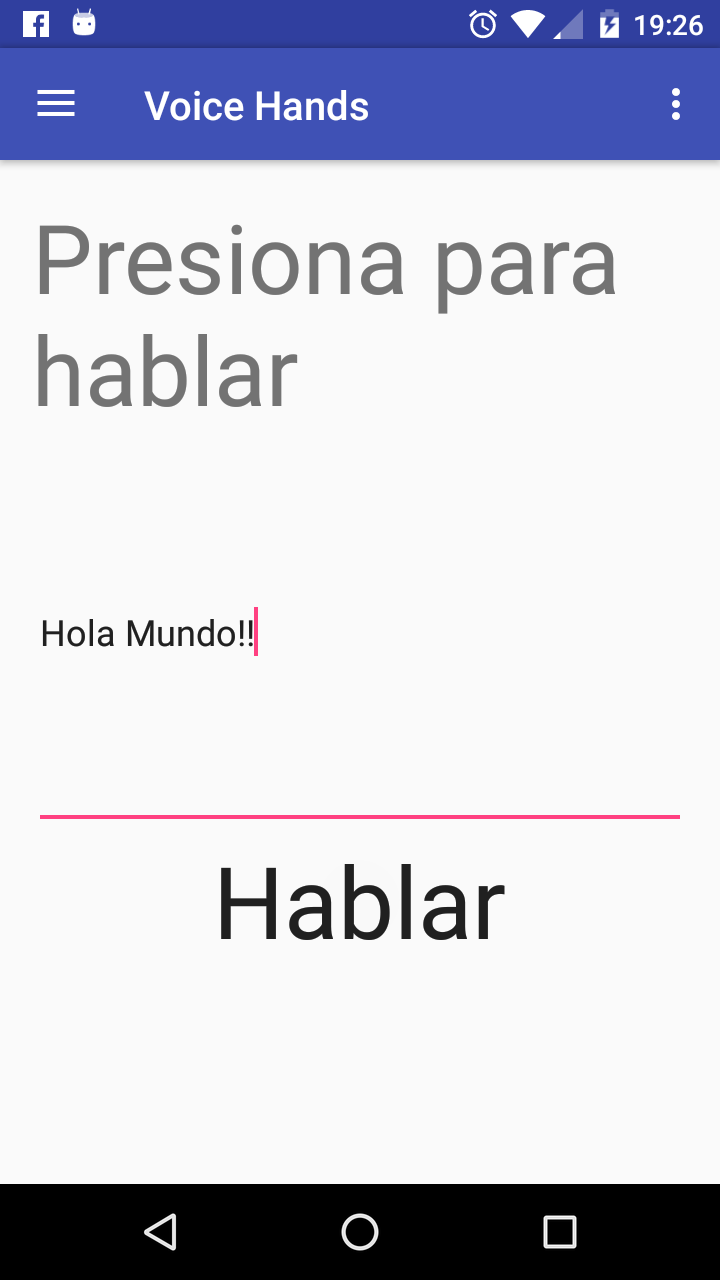
\includegraphics[scale = 0.2]{figures/app08}
	\caption{Aplicación: Reproducción de voz}
	\label{fig:app08}
\end{figure}

Finalmente se presiona el botón y a través de los altavoces se escuchará la frase.

\begin{figure}[H]
	\centering
	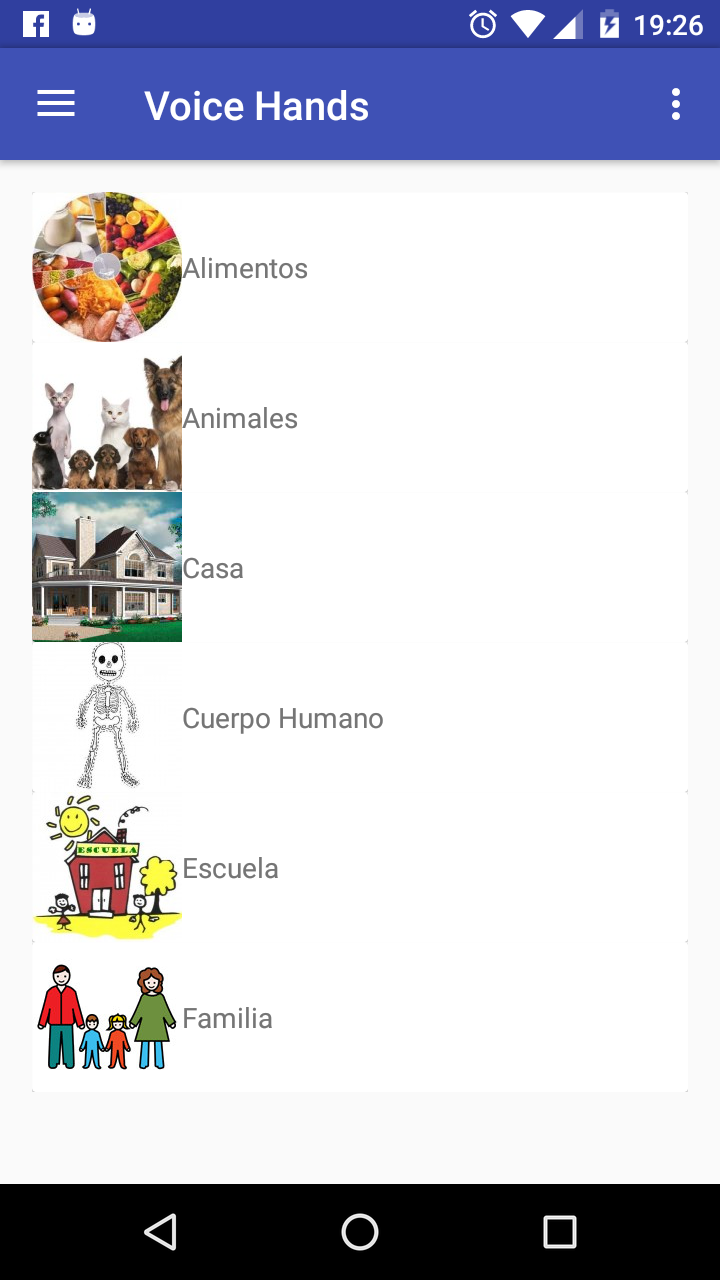
\includegraphics[scale = 0.2]{figures/app09}
	\caption{Aplicación: Categorías del diccionario}
	\label{fig:app09}
\end{figure}

Finalmente, si seleccionamos la tercera opción o el diccionario veremos esta actividad, la cual nos muestra el diccionario dividido en categorías.

\begin{figure}[H]
	\centering
	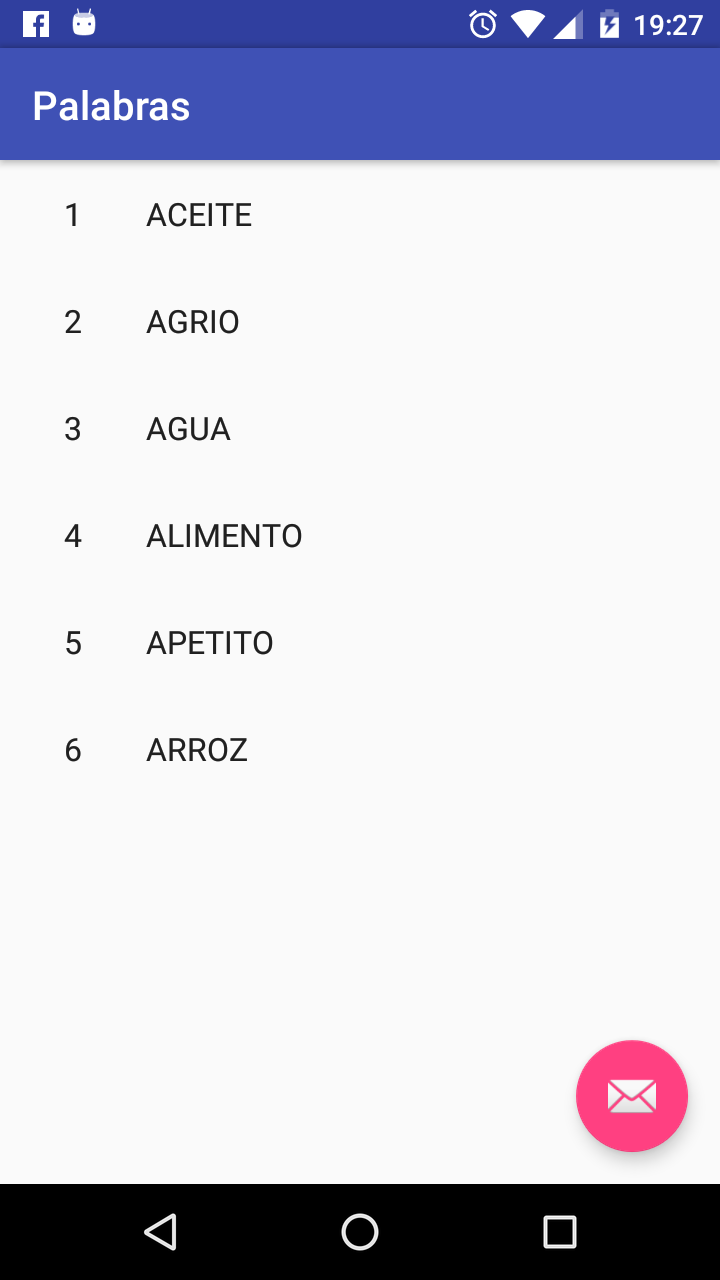
\includegraphics[scale = 0.2]{figures/app10}
	\caption{Aplicación: Palabras de una categoría}
	\label{fig:app10}
\end{figure}

Una vez seleccionada la categoría podremos seleccionar la palabra buscada o en el cuadro de texto podemos filtrar las palabras de acuerdo a lo que buscamos.

\begin{figure}[H]
	\centering
	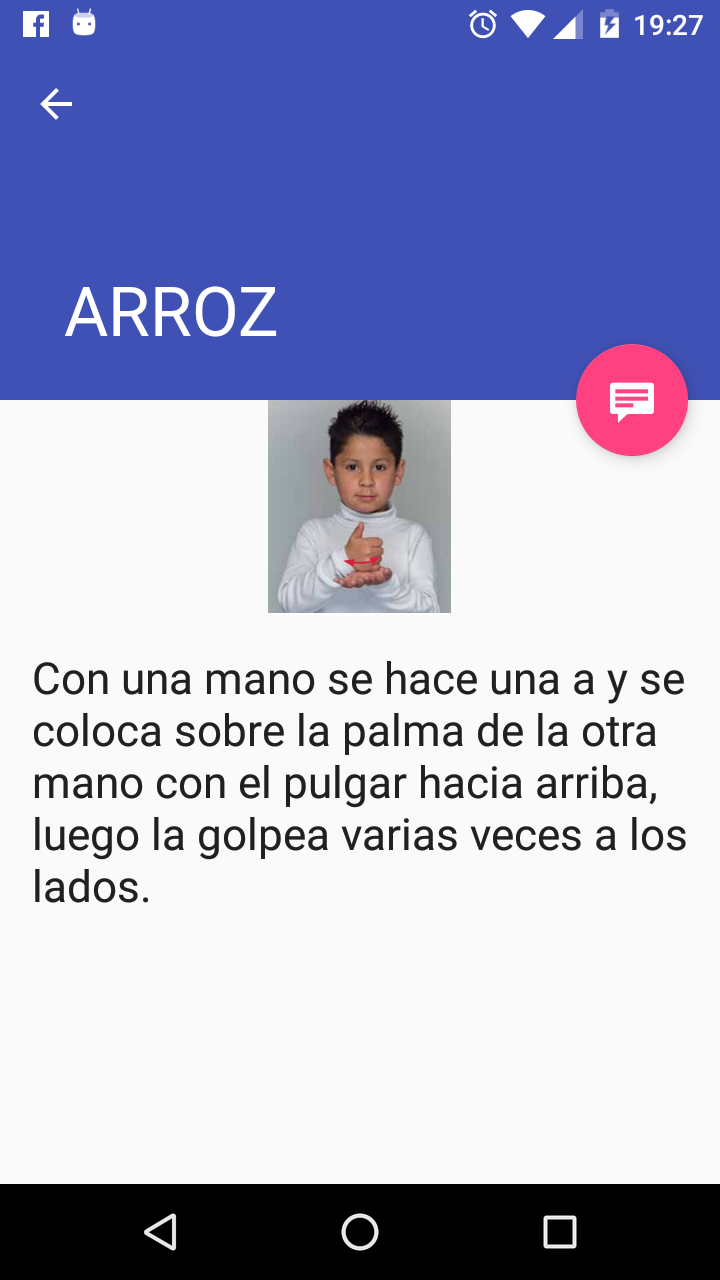
\includegraphics[scale = 0.2]{figures/app11}
	\caption{Aplicación: Información de la palabra}
	\label{fig:app11}
\end{figure}

Una vez seleccionada la palabra, la aplicación nos mostrará otra actividad con la información relacionada a ésta, tanto la seña en imagen y la instrucción para realizarla, también en algunos casos se encontrará información adicional.

%\end{multicols}